\documentclass[times]{fldauth}
%\documentclass[times,doublespace]{fldauth}

\def\volumeyear{2011}

\graphicspath{{figures/}}

\newtheorem{assumption}{Assumption}
\newtheorem{definition}{Definition}
\newtheorem{theorem}{Theorem}
\newtheorem{lemma}{Lemma}

\newtheorem{example_base}{Example}
\newenvironment{example}{\begin{example_base}}
   {\hspace{\stretch{1}}$\lozenge$\end{example_base}}

\usepackage{color}
\newcommand{\todo}[1]{\noindent\framebox{\begin{minipage}{0.97\columnwidth}\color{red}#1\end{minipage}}}

% disable todo
%\renewcommand{\todo}[1]{}


\begin{document}

\runningheads{T. Liang and M. West}{Optimized mixing in microfluidic channels}

\title{Optimized mixing in microfluidic channels}

\author{T. Liang\affil{1} and M. West\affil{2}\corrauth}

\address{\affilnum{1}Aeronautics and Astronautics,
  Stanford University, Stanford, CA 94305, USA\break
  \affilnum{2}Mechanical Science and Engineering,
  University of Illinois at Urbana-Champaign, Urbana, IL 61801, USA}

\corraddr{Email: \texttt{mwest@illinois.edu}}


%\documentclass{article}
%\usepackage{graphicx}
%\usepackage{graphicx,psfrag}
%\usepackage{graphics}
%\usepackage{amsmath}
%\usepackage{amsthm}
%\usepackage{amsfonts}
%\usepackage[margin=3cm]{geometry}
%\usepackage[margin=1.5cm,
%            vmargin={0pt,1cm},
%            nohead]{geometry}
%\title{Optimized Mixing in Microfluidic Channels}
%\author{Tzu-Chen Liang and Matthew West}
%\date{\today}
\graphicspath{{figures/}}
% End of Preamble


%\begin{document}

%%%%%%%%%%%%%%%%%%%%%%%%%%%%%%%%%%%%%%%%%%%%%%%%%%%%%%%%%%
%%%%%%%%%%%%%%%%%%%%%%%%%%%%%%%%%%%%%%%%%%%%%%%%%%%%%%%%%%
\begin{abstract}
  We develop a topology optimization method for optimizing the shape
  of pressure-driven microfluidic channels to maximize the passive
  mixing rate of advected tracers. The optimization procedure uses a
  relaxation of Stokes flow by allowing a permeable structure and the
  objective can be a function of either the fluid velocity field or
  the particle map from inlet to outlet. We present two new channel
  designs, one that is an optimized version of the herringbone mixer
  of Stroock et al., and one that mixes more quickly by using a fully
  3D structure in the channel. These channels deliver approximately
  30\% and 60\% reductions, respectively, in the 90\% mixing
  lengths. To compare our numerical simulations to experiments, we
  approximate the inlet-outlet particle map by a Markov Chain and show
  that this cheaply approximates the true stochastic map.
\end{abstract}

\keywords{Topology optimization; Microfluidic mixing; Chaotic mixing}

\maketitle

%%%%%%%%%%%%%%%%%%%%%%%%%%%%%%%%%%%%%%%%%%%%%%%%%%%%%%%%%%
%%%%%%%%%%%%%%%%%%%%%%%%%%%%%%%%%%%%%%%%%%%%%%%%%%%%%%%%%%
%
% Introduction
%
\section{Introduction}
\label{sec:topoptintro}

\paragraph{Microfluidic mixing channels.}
Microfluidic systems control and manipulate liquids in microliter or
nanoliter amounts. The study of microfluidics emerged in the 1990s and
is now widely applied in various fields such as the development of DNA
chips \cite{Burns1998}, molecular biology \cite{DavidJ2002}, chemical
reactions \cite{Andersson2000}, transfers of small volumes of
materials \cite{Sammarco1999}, and lab-on-a-chip technology
\cite{weigl2003,Stone2004}. One of the challenges in microfluidics is
the design of mixing channels, whose objective is to thoroughly mix
two or more different liquids. Although the mixers designed by using
active components like micro-pumps to stir the flow have very
promising results \cite{Yang2000,Deshmukh2000}, passive mixing devices
have advantages in manufacturing simplicity and price.

In this paper, we focus on the design and optimization of passive
microfluidic mixing channels. A microfluidic mixing channel typically
has cross-section dimension $\ell\sim 100\mu m$, and Reynolds number
$\text{Re}=U\ell/\nu$ is less than $100$ \cite{Stroock2002} ($U$ is
the average velocity of the liquid and $\nu$ is the kinematic
viscosity of the fluid).  Fluid flow on this scale is highly laminar
and the mixing of materials between streams is purely diffusive. The
dimensionless number that controls the length of the channel required
for mixing is the P\'{e}clet number ($\text{Pe}= U\ell/D$, where $D$
is the molecular diffusivity). For a pressure-driven mixing channel,
the mixing length can be expected to grow linearly with $\text{Pe}$
and is usually much more than $1\,\text{cm}$. Hence various designs
have been proposed to stir the flow inside the channel and produce
transverse velocities to enhance the mixing \cite{Stroock2002,
  Ottino2004Science, Wiggins2004}.

The mixing problem has been linked to chaotic mixing protocols, which
are believed to have the best mixing results due to the stretching and
folding features of chaotic maps. A typical way to realize chaotic
mixing is through the design of linked twist
maps~\cite{Wiggins2004}. However, there is no direct way to realize
the designed linked twist map in a mixing channel, either by passive
structures or active mechanisms such as variable-frequency pumps or
internal moving components. In this paper, we use the techniques
developed in topology optimization to find the internal structure of a
mixing channel to realize a desired flow field or flow map. The
results can be applied to mixing channel design when the desired
mixing protocol is known.


\paragraph{Topology optimization.}
A typical topology optimization problem is to distribute a given
amount of material in a design domain, subject to load and support
conditions, such that the stiffness of the structure is maximized
\cite{Bendsoe2003}. The design parameters are usually the spatial
distribution of the material. Even though the optimal solution is in
general quite sparse in space, the number of variables is often
inevitably large in the formulation. Some problems, such as truss
topology design, can be formulated as convex optimization problems
\cite{BenTal1997} by relaxing the material density to be variable, and
are thus solvable by efficient algorithms. The optimal solution of the
relaxed optimization is shown to be a black/white solution and thus
also the optimal solution of the original problem. In other cases when
the problem has no convex formulation, nonlinear optimization
techniques need to be applied and it is in general hard.

Topology optimization has been applied to the design of optimal shapes
of pipes or diffusers such that the total potential power drop is
minimized \cite{Evgrafov2005, Borrvall2003}. In that work, Darcey flow
is used to simulate the flow inside porous material and form a
relaxation. The design parameters in this formulation are the
permeability of the material on a spatial grid. In this case, the
relaxed problem is still non-convex, but can be solved by means of
sequential separable and convex programming. A two-step solution
procedure is thus applied to find a black/white solution with
permeability either $0$ or infinity at a point.

In this paper we use the same relaxation strategy \cite{Evgrafov2005,
  Borrvall2003} to formulate the mixing channel design as a topology
optimization problem. We assume that our mixing channel is a periodic
repetition of a basic block, which is what we optimize. We use a proxy
objective function that is a function of the velocity field or a map
between the inlet and the outlet of one period of the channel. These
proxy cost functions are chosen so that optimizing them produces the
desired mixing or other flow behavior. This results in a nonlinear
optimization problem and a sub-gradient method is developed to find
the local minimum of the objective function. We do not consider the
fabrication issue explicitly when solving the topology optimization
problem.

\paragraph{The simulation of advection-diffusion equations.}
Another challenge in the design of microfluidic mixing channels is
that there is no clear measure of how well a channel mixes. In
experiments it is common to measure the variance of colored liquids on
the cross-section of the channel to see how well they are mixed
\cite{Stroock2002}. However, when doing simulation, this corresponds
to solving the advection-diffusion equation for a 3D flow field in a
very long channel with very small diffusion, which is extremely
expensive. The problem is that the relationship between the channel
structure and the resulting variance of the liquid on a cross-section
is very complicated.

In this paper, we develop a Markov Chain model to approximate the
mixing process from one channel cross-section to the next, using a
high resolution 2D grid. Similar approaches can be found in, for
example, \cite{Dellnitz1999, Dellnitz2002, Froyland1998, Froyland1999,
  Froyland2001}. This is a cheap way to replace the solution of the
advection-diffusion equation and can let one observe the mixing
process and measure the variance of the colored field easily. This
model does not represent a high-fidelity solution of the
advection-diffusion equation, but it captures the most important
factors of the chaotic mixing: stretching, folding and molecular
diffusion. In addition, because we can use a high resolution 2D grid,
we can keep numerical diffusivity below the physical diffusivity.

\paragraph{Outline of the paper.}
In Section~\ref{sec:opt} we describe the mathematical model of mixing
channels and how to form the topology optimization problem using a
relaxation of Stokes flow to Darcy flow. Section~\ref{sec:simu}
discusses the simulation issue and a Markov chain model is proposed to
approximate the solution of the advection-diffusion equation to evolve
the color intensity field. Results are given in
Section~\ref{sec:topoptresults} and finally conclusions are in
Section~\ref{sec:topoptconclusion}.

%%%%%%%%%%%%%%%%%%%%%%%%%%%%%%%%%%%%%%%%%%%%%%%%%%%%%%%%%%
%%%%%%%%%%%%%%%%%%%%%%%%%%%%%%%%%%%%%%%%%%%%%%
%%%%%%%%%%%%%%%%%%%%%%%%%%%%%%%%%%%%%%%%%%%%%%
\section{Forming the optimization problem}
\label{sec:opt}
%%%%%%%%%%%%%%%%%%%%%%%%%%%%%%%%%%%%%%%%%%%%%%
%%%%%%%%%%%%%%%%%%%%%%%%%%%%%%%%%%%%%%%%%%%%%%

%%%%%%%%%%%%%%%%%%%%%%%%%%%%%%%%%%%%%%%%%%%%%%
\subsection{Mathematical model of a periodic microfluidic mixing channel}
%%%%%%%%%%%%%%%%%%%%%%%%%%%%%%%%%%%%%%%%%%%%%%

We are concerned with mixing in a long and thin channel. Fluids with
two different colors (represented by intensities $1$ and $0$) are
injected in one end of the channel and flow through it, driven by body
force only. The channel has some internal structure that acts to stir
the fluid passively. This structure is periodic with period $\ell_x$
and the cross-section of the channel has dimension $\ell_y$ by
$\ell_z$. The channel is assumed to be long enough so that the
velocity field inside is fully developed and hence also periodic with
period $\ell_x$. Because of the periodic velocity field, we need to
solve it for only one period, and we can then use this velocity field
to transport the fluid with different colors iteratively to observe
the mixing process. In fact, we calculate the streamlines that connect
the two ends ($x=0$ and $x=\ell_x$) of one period length channel and
define a Poincar\'e map. Applying this map repeatedly tells us how a
particle moves between different cross-sections along the channel.

\begin{figure}
  \centerline{
    \begin{picture}(350,150)
      \put(0,0){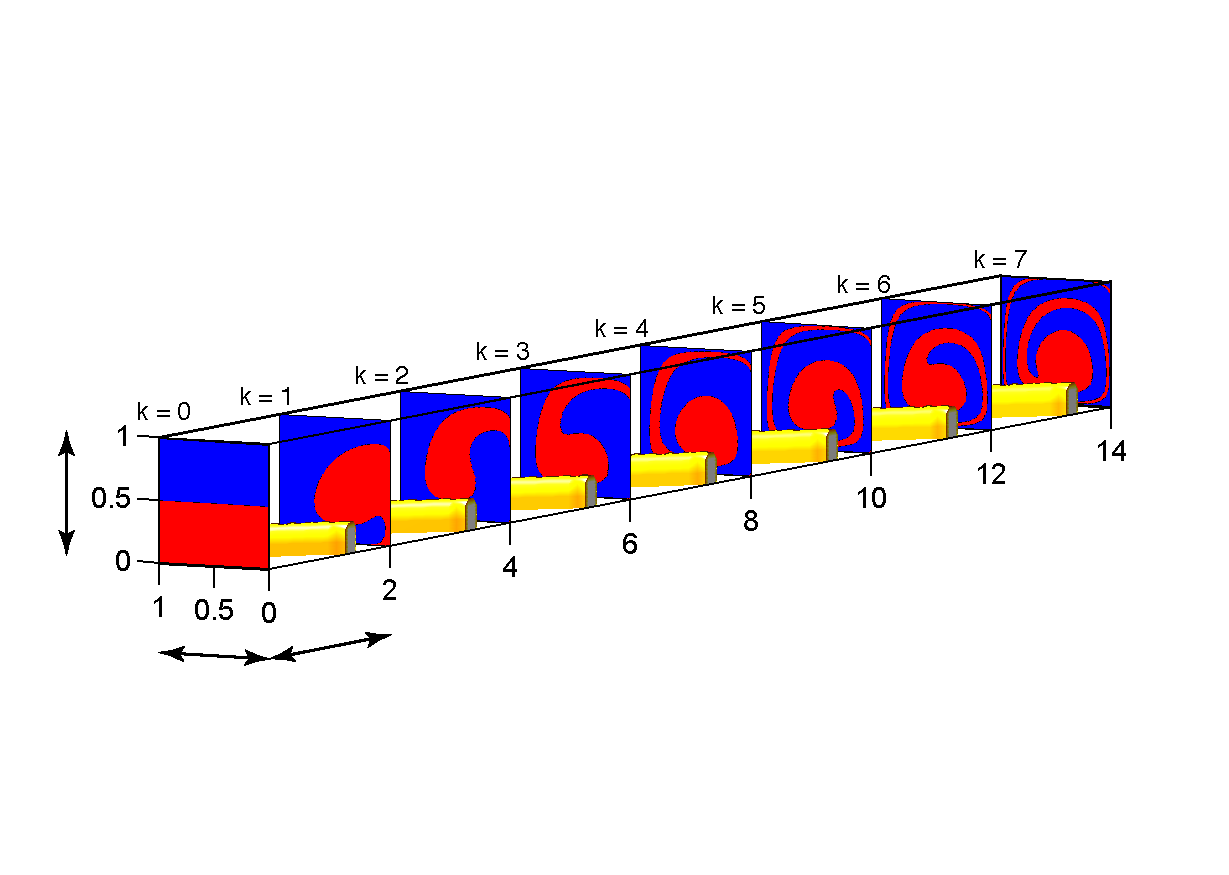
\includegraphics[width=0.8\textwidth,trim=0.5cm 2.9cm 1.5cm 4.1cm,clip]{mixingchannel}}
      \put(55,5){$\ell_z$}
      \put(95,8){$\ell_x$}
      \put(-1,67){$\ell_y$}
    \end{picture}
    }
    \caption{\label{mixingchannel} The mixing channel. Liquids with
      two different colors are originally separate and injected from
      one end of the channel. The channel consists of repeats of a
      periodic block of size $\ell_x \times \ell_y \times \ell_z$
      containing structures to alter the flow and produce mixing of
      the colored liquids. In this figure, cross-sections of the color
      distribution are plotted every period of the structure ($k = 0$
      to $k = 7$).}
\end{figure}

As mentioned in the introduction, flow on the microfluidic
scale has $\text{Re}\sim 1$ and is thus highly laminar. A Stokes partial
differential equation is generally a reasonable model of the motion.
We simulate the flow by the generalized Stokes equation for
incompressible flow:
\begin{subequations}
  \label{stokes}
  \begin{align}
    \label{stokes1}
    ( -\nu\Delta + \alpha)u
    + \nabla p &= b, \\
    \label{stokes2}
    \operatorname{div} u &= 0,
  \end{align}
\end{subequations}
where $u(\mathbf{x})$ and $p(\mathbf{x})$, which are both functions of
position $\mathbf{x}=(x,y,z)$, stand for the velocity and pressure
fields and $b$ is the body force that drives the flow. It has an
elliptic operator $-\nu\Delta + \alpha $ in which $\nu$ is the
kinematic viscosity and $\alpha(\mathbf{x})$ represents the inverse
permeability at $\mathbf{x}$. When $\alpha(\mathbf{x}) = 0 $ it is
just Stokes flow with viscosity $\nu$ and when $\nu=0$, one obtains
the Darcy equation, which governs the flow in porous material with
permeability $\alpha^{-1}$. This represents a relaxation of the true
problem~\cite{Evgrafov2005, Borrvall2003}, which is presumed to use
impermeable material with $\alpha = \infty$. As we will discuss in
Section~\ref{sec:maxim-downw-veloc}, in practice we find that optimal
designed typically have $\alpha$ either very low or very high, which
we then take to be zero or infinite, respectively.

The liquids to be mixed are assumed to have the same density and
viscosity, which is true for many applications when the liquids are
solvents carrying different reactants. This assumption is critical for
our periodic setting to work, because now we can separate the color
intensity field from the velocity field: the velocity field is
stationary and periodic but the color intensity field is not. This
allows us to use one period of velocity field repeatedly to carry the
color intensity and observe the mixing process.

We use a finite-difference method with staggered regular meshes to
solve the above equation. Assuming the finite-dimensional
approximation of the Laplace, gradient and divergence operators on the
given mesh are $L$, $G$, and $D$, the generalized Stokes equation can
be represented by
\begin{equation}
  \label{discretestokes}
  \begin{bmatrix}
      -\nu L + \text{diag}(\bar{\alpha})H & G \\
             D                            &  0
    \end{bmatrix}
  \begin{bmatrix}
      \bar{u} \\ \bar{p}
    \end{bmatrix} =
  \begin{bmatrix}
      \bar{b} \\ \mathbf{0}
    \end{bmatrix},
\end{equation}
where $\bar{u}$, $\bar{p}$, $\bar{\alpha}$, and $\bar{b}$ are vectors,
representing finite-dimensional approximations of $u$, $p$, $\alpha$
and $b$, respectively. The linear operator $H$ maps the design
parameters $\bar{\alpha}$ to the directional $\bar{u}$ grids.

Let the number of grid cells in the $x$, $y$, and $z$ directions be
$n_x$, $n_y$, and $n_z$. We define $n_{\bar{u}} = 3n_x n_y n_z$, which
is roughly the size of $\bar{u}$, and $n_{\bar{\alpha}}=n_{\bar{p}} =
n_x n_y n_z$, which is roughly the size of $\bar{\alpha}$ and
$\bar{p}$ (boundary conditions make these expressions only
approximate). A typical case in our examples is $n_x = 144$, $n_y=24$,
and $n_z=48$.

%%%%%%%%%%%%%%%%%%%%%%%%%%%%%%%%%%%%%%%%
\subsection{Topology optimization}
%%%%%%%%%%%%%%%%%%%%%%%%%%%%%%%%%%%%%%%%

We would like to optimize some objective function
$g(\bar{u},\bar{p},\bar{\alpha})$ over parameters $\bar{\alpha}$. The
direct approach would be to define an optimization problem
\begin{subequations}
\begin{align}
  \text{minimize } &g(\bar{u},\bar{p},\bar{\alpha}) \\
  \label{eqn:stokes_constraint}
  \text{subject to } &\begin{bmatrix} -\nu L + \text{diag} (\bar{\alpha}) H
       & G \\ D & 0
    \end{bmatrix}
    \begin{bmatrix}
      \bar{u} \\ \bar{p}
    \end{bmatrix} =
    \begin{bmatrix}
     \bar{b} \\ \mathbf{0}
    \end{bmatrix}, \\
    &0 \le \bar{\alpha} \le \alpha_{\text{max}},
\end{align}
\end{subequations}
where $\alpha_{\text{max}}\in \mathbb{R}$ is a large number to
approximate the minimum permeability when $\alpha$ goes to infinity
and the structure is solid. The optimization problem has variables
$\bar{u}$, $\bar{p}$, and $\alpha_{\text{max}}$, and a large set of
nonlinear equality constraints that make the problem extremely hard to
solve.

For a given $\bar{\alpha}$, we can solve \eqref{eqn:stokes_constraint}
to obtain $\bar{u}$ and $\bar{p}$ and there are no inequality
constraints on these two variables. We can thus rewrite the
optimization and lump the equality constraints into the objective
function:
\begin{subequations}
  \label{topoptform}
  \begin{align}
    \label{topoptform_cost}
    \text{minimize } &g(\bar{u}(\bar{\alpha}),
    \bar{p}(\bar{\alpha}), \bar{\alpha}) \\
    \label{topoptform_constraint}
    \text{subject to } &0\le \bar{\alpha} \le \alpha_\text{max}.
  \end{align}
\end{subequations}
This formulation reduces the number of variables and eliminates the
nonlinear equalities, but it is now harder to evaluate the gradient of
the objective function, which we desire for efficiency in the
optimization algorithm. We will show later that an adjoint method can
be applied to efficiently compute the gradient.

%%%%%%%%%%%%%%%%%%%%%%%%%%%%%%%%%%%%%%%%%%%%%%%%%%%%%%%%
\subsection{Objective functions and a descent direction}
%%%%%%%%%%%%%%%%%%%%%%%%%%%%%%%%%%%%%%%%%%%%%%%%%%%%%%%%

%%%%%%%%%%%%%%%%%%%%%%%%%%%%%%%%%
\paragraph{Objective functions.}
%%%%%%%%%%%%%%%%%%%%%%%%%%%%%%%%%
Our goal is to optimize the shape of the structure inside the channel.
That is, to find a vector $\bar{\alpha}$ such that the function
$g(\bar{u},\bar{p},\bar{\alpha})$ is locally minimized. The ideal
objective function is mixing length \cite{Stroock2002}: the channel
length required for the standard deviation of the color intensity on
the cross-section to drop by a given ratio. Unfortunately, this is a
very complicated function of the channel structure and there is no
clear way to find a descent direction to improve it. Hence, we use
several steps of heuristic designs to reduce the mixing length.

Two types of objective function will be considered in our
formulation. The first one is a function of the velocity field, which
is a very direct way to design the flow. In fact, for most
applications, a linear function is sufficient:
\begin{align}
  \label{g1}
  g_1(\bar{u},\bar{p},\bar{\alpha}) = \bar{c}^T\bar{u},
\end{align}
for a given vector $\bar{c}$.

The second type of objective function measures the difference between
two maps. For a given velocity field $u$, the streamlines can be
calculated by numerical integration. Each of the streamlines connects
a point on the $y$-$z$ plane at $x=0$ to another point at
$x=\ell_x$. The streamlines thus define an end-to-end flow map
$S_u:[0,\ell_y]\times[0,\ell_z] \to
[0,\ell_y]\times[0,\ell_z]$. Define $g_2(u,p,\alpha;S^*) = \|S^* -
S_u\|$, where $S^*: [0,\ell_y] \times [0,\ell_z] \to [0,\ell_y] \times
[0,\ell_z]$ is the desired end-to-end flow map and $\| \cdot \|$ is a
norm on scalar maps (which could be relaxed to a distance
function). Suppose we know the desired map $S^*$. The second type of
objective function can then be applied to minimize the difference
between the current map and the desired map. However, because each
streamline needs to be calculated numerically, to define a map would
be extremely hard. Therefore we simplify this objective function and
let it measure the difference between a set of sample points on the
$y$-$z$ plane. Let $(\bar{y}_0,\bar{z}_0)$ be a set of sample points
on the $y$-$z$ plane at $x=0$. We have
\begin{align*}
  (\bar{y}_e^*,\bar{z}_e^*)&= S^*(\bar{y}_0,\bar{z}_0), \\
  (\bar{y}_e,\bar{z}_e)    &= S_u(\bar{y}_0,\bar{z}_0). 
\end{align*}
We simply define $g_2$ as
\begin{eqnarray}
  \label{g2}
  g_2(u,p,\alpha;S^*,\bar{y}_0,\bar{z}_0)
  = \|\bar{y}_e^*-\bar{y}_e\|^2 + \|\bar{z}_e^*-\bar{z}_e\|^2,
\end{eqnarray}
where $\|\cdot\|$ is the $2$-norm of a vector. The above function is a
rough measure of how close the maps $S_u$ and $S^*$ are. In our
examples, $(\bar{y}_0,\bar{z}_0)$ is chosen as a regular grid of
points in the $y$-$z$ plane.

%%%%%%%%%%%%%%%%%%%%%%%%%%%%%%%%%%%%%%%%%%%%%%%%%%%%%%%%%%%%%%%%%%%%
\paragraph{Adjoint method for $d g_1/d \mathbf{\bar{\alpha}} $.}
%%%%%%%%%%%%%%%%%%%%%%%%%%%%%%%%%%%%%%%%%%%%%%%%%%%%%%%%%%%%%%%%%%%%
To find a descent direction of $g_1$ with respect to $\bar{\alpha}$,
the adjoint method \cite{Jameson1999} is applied. Let $\bar{v} =
[\bar{u}^T\ \bar{p}^T]^T$. The variables $\bar{v}$ and $\bar{\alpha}$
satisfy a set of constraints $R(\bar{v},\bar{\alpha})=0$ defined
by~(\ref{discretestokes}). If we directly
differentiate~(\ref{topoptform_cost}) with respect to $\bar{\alpha}$
using the chain rule, then it will be necessary to compute
$d\bar{v}/d\bar{\alpha}$. Unfortunately, $d\bar{v}/d\bar{\alpha}$ has
size $(n_{\bar{u}}+n_{\bar{p}}) \times n_{\bar{\alpha}}$ (very large)
and is dense. We would like to calculate $d g_1/d\bar{\alpha}$ without
explicitly forming $d\bar{v}/d\bar{\alpha}$. The adjoint
method~\cite{Errico1997} is designed for this situation. We begin with the
total derivative of $g_1$ and $R$ with respect to $\alpha$:
\begin{align*}
  \frac{dg_1}{d\bar{\alpha}} &=
  \frac{\partial{g_1}}{\partial{\bar{\alpha}}}+
  \frac{\partial{g_1}}{\partial{\bar{v}}} \frac{d\bar{v}}{d\bar{\alpha}},\\
  \frac{dR}{d\bar{\alpha}} &=
  \frac{\partial{R}}{\partial{\bar{\alpha}}}+
  \frac{\partial{R}}{\partial{\bar{v}}}
  \frac{d\bar{v}}{d\bar{\alpha}}=0.
\end{align*}
From the second equation, we have
\begin{equation*}
  \frac{d\bar{v}}{d\bar{\alpha}}
  = -\left(\frac{\partial{R}}{\partial{\bar{v}}}\right)^{-1}
  \frac{\partial{R}}{\partial{\bar{\alpha}}}.
\end{equation*}
Substituting this into the first equation gives:
\begin{equation*}
   \frac{dg_1}{d\bar{\alpha}}
   = \frac{\partial{g_1}}{\partial{\bar{\alpha}}}
   -\frac{\partial{g_1}}{\partial{\bar{v}}}
   \left(\frac{\partial{R}}{\partial{\bar{v}}}\right)^{-1}
   \frac{\partial{R}}{\partial{\bar{\alpha}}}.
\end{equation*}
Let $\Phi = -\frac{\partial{g_1}}{\partial{\bar{v}}}
\left(\frac{\partial{R}}{\partial{\bar{v}}}\right)^{-1}$. Then
$\Phi$ satisfies
\begin{equation}
\label{adjointeq}
 \Phi \frac{\partial{R}}{\partial{\bar{v}}}
 = -{\frac{\partial{g_1}}{\partial{\bar{v}}}}.
\end{equation}
The above equation is called the adjoint equation. More explicitly,
the adjoint equation in our formulation is
\begin{equation}
\label{adjointeq2}
  \begin{bmatrix}
     -\nu L + \text{diag}(\bar{\alpha})H   & G\\
     D               &  0
   \end{bmatrix}^T \Phi^T =
  \begin{bmatrix}
    -\big(\frac{\partial{g_1}}{\partial{\bar{u}}}\big)^T\\
    0
   \end{bmatrix}.
\end{equation}
After solving for $\Phi$, we can then evaluate $dg_1/d\bar{\alpha}$ by
\begin{equation}
\label{dg1dalpha}
  \frac{dg_1}{d\bar{\alpha}}
  = \frac{\partial{g_1}}{\partial{\bar{\alpha}}}
  + \Phi \frac{\partial{R}}{\partial{\bar{\alpha}}}.
\end{equation}
In our problem, $g_1$ does not depend on $\bar{\alpha}$ explicitly, so
the first term in the right-hand side of (\ref{dg1dalpha}) is zero. To
solve the adjoint equation (\ref{adjointeq2}), we need
$\partial{g_1}/\partial{\bar{u}}$, which is just $\bar{c}^T$ for
$g_1$. Note that solving~(\ref{adjointeq2}) and
evaluating~(\ref{dg1dalpha}) have a similar cost to
solving~(\ref{discretestokes}), which is dramatically less than the
cost of forming $d\bar{v}/d\bar{\alpha}$.

%%%%%%%%%%%%%%%%%%%%%%%%%%%%%%%%%%%%%%%%%%%%%%%%%%%%%%%
\paragraph{Streamlines and $\partial g_2/\partial {\bar{u}}$.}
%%%%%%%%%%%%%%%%%%%%%%%%%%%%%%%%%%%%%%%%%%%%%%%%%%%%%%%
To find $d g_2/d \bar{\alpha}$, the above approach is still valid but
we need to form $\partial{g_2}/\partial{\bar{u}}$ first. Let the
solution of (\ref{discretestokes}) be the discrete velocity field
$\bar{u} = [\bar{u}_{x}^T\ \bar{u}_{y}^T\ \bar{u}_{z}^T]^T$. The velocity at
any point can be evaluated by linear interpolation. Given an initial
point $(0,y_{0},z_{0})$, a second-order Runge-Kutta method is applied to
find the streamline passing through it. Because both the interpolation
and Runge-Kutta method have linear weights on $\bar{u}$, we can write
down the following relations:
\begin{align*}
 x_e & = k_{x}^T \bar{u}_{x}+0,\\
 y_e & = k_{y}^T \bar{u}_{y}+y_{0},\\
 z_e & = k_{z}^T \bar{u}_{z}+z_{0},
\end{align*}
where $k_{x}$, $k_{y}$ and $k_{z}$ are the constant weighting vectors
generated by the numerical integration. We set $(x_e,y_e,z_e)$ to be
the point that $(0,y_{0},z_{0})$ is transported to, assuming $x_e=
\ell_x$.  Then $dy_e/d\bar{u}$ and $dz_e/d\bar{u}$ can be written as
\begin{align}
\begin{split}
 \frac{dy_e}{d\bar{u}}
 &=  \left[ \frac{\partial{y_e}}{\partial{x_e}}
   \frac{dx_e}{d\bar{u}_{x}},
   \frac{dy_e}{d\bar{u}_{y}},
   \mathbf{0}^T\right]
 = \left[\frac{u_y(\mathbf{x}_e)}{u_x(\mathbf{x}_e)}k_{x}^T,
   k_{y}^T ,\mathbf{0}^T \right], \\
 \frac{dz_e}{d\bar{u}}
 &=  \left[ \frac{\partial{z_e}}{\partial{x_e}}
   \frac{dx_e}{d\bar{u}_{x}},
   \mathbf{0}^T,
   \frac{dz_{e}}{d\bar{u}_{z}}\right]
 = \left[\frac{u_z(\mathbf{x}_e)}{u_x(\mathbf{x}_e)}k_{x}^T,
   \mathbf{0}^T, k_{z}^T \right],
\end{split}
\end{align}
where $\mathbf{x}_e= (x_e,y_e,z_e)$ and $u_x(\mathbf{x}_e)$,
$u_y(\mathbf{x}_e)$ and $u_z(\mathbf{x}_e)$ can also be evaluated by
interpolation. Hence $dg_2/d\bar{u}$, where $g_2$ has the form of
equation (\ref{g2}), can be written as
\begin{align}
  \frac{\partial g_2}{\partial \bar{u}}
  = \sum_{y_e} \frac{\partial{g_2}}{\partial{y_e}}
  \frac{dy_e}{d\bar{u}}
  + \sum_{z_e}
  \frac{\partial{g_2}}{\partial{z_e}}\frac{dz_e}{d\bar{u}}.
\end{align}

%%%%%%%%%%%%%%%%%%%%%%%%%%%%%%%%%%%%%%%%%%%%%%%%%%%%%%%%
\subsection{The gradient-based optimization method}
\label{sec:grad-based-optim}
%%%%%%%%%%%%%%%%%%%%%%%%%%%%%%%%%%%%%%%%%%%%%%%%%%%%%%%%

We use a gradient-based method to solve (\ref{topoptform}):
\begin{center}
  \begin{tabular}{ll}
    \multicolumn{2}{l}{\textbf{Topology Optimization Algorithm}} \\
    \hline
    \textbf{given}
    & a starting vector $\bar{\alpha}^0$ \\
    & iteration number $i=0$ \\
    & cost function $g = g_1$ or $g_2$ \\
    & a gradient step scale $\delta$ \\[0.5em]
    \textbf{repeat}
    & 1. solve (\ref{discretestokes}) for the velocity field
    $\bar{u}$ and pressure field $\bar{p}$ \\
    & 2. solve the adjoint equation (\ref{adjointeq2}) and find
    $\frac{dg}{d\bar{\alpha}}$ \\
    & 3. $\bar{\alpha}^{i+1} = 
    \bar{\alpha}^{i} - \delta \frac{dg}{d\bar{\alpha}}$ \\
    & 4. project the components of $\bar{\alpha}^{i+1}$ outside
    $[0,\alpha_\text{max}]$ to $0$ and $\alpha_\text{max}$ \\
    & 5. $i = i+1$ \\[0.5em]
    \textbf{until}
    & stopping criterion is satisfied \\
    \hline
  \end{tabular}
\end{center}
For all of our examples, we use $\bar{\alpha}^0 = \mathbf{0}$ as the
initial material distribution, and we do not impose a total material
constraint. In step $4$ of the algorithm, the clipping of
$\bar{\alpha}$ to zero is necessary because material with negative
inverse permeability does not make physical sense.

In our formulation, to evaluate the objective function is very
expensive, so there is no line search in this algorithm. A fixed step
size is used, and the step size is tuned by hand in our examples. The
stopping criterion we use is
\begin{align}
  \left\|\frac{\bar{\alpha}^i}{\|\bar{\alpha}^i\|_2}
    - \frac{\bar{\alpha}^{i+1}}{\|\bar{\alpha}^{i+1}\|_2}\right\|_2
  < \epsilon.
\end{align}
For all of our examples, we observe that when the structure is formed,
the projection of the negative gradient direction gradually aligns
with the current $\bar{\alpha}^i$ direction. So the structure shape
does not change but the permeability keeps decreasing. Hence this stop
criterion performs well in finding the optimal structure shape.

%%%%%%%%%%%%%%%%%%%%%%%%%%%%%%%%%%%%%%%%%%%%%%%%%%%%%%%%%%%%%%%%%%%%%%
%%%%%%%%%%%%%%%%%%%%%%%%%%%%%%%%%%%%%%%%%%%%%%%%%%%%%%%%%%%%%%%%%%%%%%
\section{Simulation of mixing in the channel}
\label{sec:simu}
%%%%%%%%%%%%%%%%%%%%%%%%%%%%%%%%%%%%%%%%%%%%%%%%%%%%%%%%%%%%%%%%%%%%%%
%%%%%%%%%%%%%%%%%%%%%%%%%%%%%%%%%%%%%%%%%%%%%%%%%%%%%%%%%%%%%%%%%%%%%%

Consider a channel design consisting of a $k$ repetitions of a channel
block of dimensions $\ell_x \times \ell_y \times \ell_z$. We assume,
as above, that the flow in the channel is also periodic and
satisfies~(\ref{stokes}). We want to know how separate fluids injected
at the channel inlet mix by the time they reach the channel outlet. We
let $Y = [0,\ell_y]\times[0,\ell_z]$ the channel cross-section between
each channel block and we represent the fluid color on the $k$th
cross-section by a scalar function $f^k : Y \to \mathbb{R}$, with $f$
taking values from $0$ to $1$. We will take $f^0$ to be
\begin{align}
  f^0(y,z) = \begin{cases} 0 & z < \ell_z/2 \\
    1 & z \ge \ell_z/2
  \end{cases}
\end{align}
and we want to compute the successive color cross-sections $f^k$, as
illustrated in Figure~\ref{mixingchannel}. Ideally, we would solve the
advection-diffusion equation
\begin{align}
  \label{ade}
  u \cdot \nabla \phi &= D \Delta \phi
\end{align}
with appropriate boundary conditions for the scalar color
$\phi(\mathbf{x})$, so that $f^k(y,z) = \phi(k\ell_x,y,z)$ for each
$k$. Solving~(\ref{ade}) is significantly more expensive than solving
for the periodic flow field, as the flow field is only solved on a
domain of size $\ell_x \times \ell_y \times \ell_z$, while $\phi$ is
not periodic and so~(\ref{ade}) would need to be solved on a domain of
size $(k \ell_x) \times \ell_y \times \ell_z$ for $k$ up to $k = 300$
or more. In addition, a very fine grid would be needed to
solve~(\ref{ade}) to avoid having the numerical diffusion from the
discretization dominate the physical diffusion.

Instead of solving~(\ref{ade}), we approximate the solution by
constructing the particle advection map $S : Y \to Y$ for a single
channel period, and a diffusion operator $\Psi_D(f)$ corresponding to
convolution with a Gaussian to give the diffusion of $f$ with
diffusivity $D$. Then we approximate the evolution of $f^k$ by
\begin{align}
  \label{eqn:periodic_f_evolution}
  f^{k+1} = \Psi_D(f^k \circ S^{-1}).
\end{align}
This approximation lumps the diffusion into the end of each channel
periodic block and assumes that all streamlines experience the same
diffusion. In reality, streamlines with lower velocities will have
longer transport times, so will experience higher diffusion. We do not
account for this effect in our approximation, as variations in
advection dominate variations in diffusion for spatially variable
mixing rates.

This approximation is both much cheaper than solving~(\ref{ade}), and
also more accurate for any feasible grid resolutions. This is because
we only need to discretize the channel cross-sections to
compute~(\ref{eqn:periodic_f_evolution}), so we can use a very high
resolution 2D mesh and keep the numerical diffusion well below the
physical diffusion. With the 3D advection-diffusion
equation~(\ref{ade}) this would be infeasible.

%%%%%%%%%%%%%%%%%%%%%%%%%%%%%%%%%%%%%%%%%%%%%
\subsection{Numerical approximation of advection}
%%%%%%%%%%%%%%%%%%%%%%%%%%%%%%%%%%%%%%%%%%%%%

To formalize the advection of the color tracer by the fluid flow, we
define the function advection operator on $Y$ corresponding to the map
$S$ is as follows.

\begin{definition}[Koopman operator]
  Let $f : Y \to \mathbb{R}$. The \emph{Koopman operator} $U_S$
  associated to $S$ gives $U_S f : Y \to \mathbb{R}$ defined by
 \begin{align}
   U_S f = f \circ S,
 \end{align}
so $(U_S f)(y,z) = f(S(y,z))$.
\end{definition}
The Koopman operator evolves scalar functions on $Y$. As we see
from~(\ref{eqn:periodic_f_evolution}), the advection of $f^k$
downstream to $f^{k+1}$ occurs by the Koopman operator $U_{S^{-1}}$ of
$S^{-1}$. We note that the following conservation holds:
\begin{equation}
\label{fvc}
  \iint_Y f^k(y,z) u_x(y,z) \,dy\,dz = \iint_Y (U_{S^{-1}} f^k)(y,z) u_x(y,z) \,dy\,dz,
\end{equation}
where $u_x: Y \to \mathbb{R}$ is the stationary $x$-component of
velocity on the cross-sections $x=0, \ell_x, 2\ell_x, \ldots$, and
this can be shown to be an invariant measure of $S$. This conservation
equation expresses the fact that the total ``color'' flowing in and
out of each period of the channel is constant.

We discretize the cross-section $Y$ into a regular grid with $m = m_y
\times m_z$ grid cells $a_1,a_2,\ldots,a_m$ of size $h \times h$, so a
scalar function $f$ on $Y$ can be approximated by its value $(f_m)_i$
on each grid cell $a_i$, giving a vector $f_m \in \mathbb{R}^m$.

We find the discrete Koopman operator $U_{S^{-1},m}$ using optimal
prediction model reduction \cite{ChorinHald2, ChorinHald1,
  mori1965tcm, zwanzig1980pnt, evans2008smn, Froyland2001,
  Froyland1999} (see~\cite{BeLaLiWe2009} for an overview in the finite
dimensional setting), as described in~\cite{numcutoff}. The discrete
optimal predictor $U_{S^{-1},m}$ for the Koopman operator $U_{S^{-1}}$
can be shown~\cite{numcutoff} to have matrix form
\begin{align}
  \label{eqn:opt_predict_Koopman}
  (U_{S^{-1},m})_{ij}
  = \frac{\displaystyle \int_{S(a_j) \cap a_i}
    \bar{\omega}(y,z)\,dy\,dz}{\displaystyle
    \int_{a_j} \bar{\omega}(y,z)\,dy\,dz},
\end{align}
where $\bar{\omega}$ is the invariant distribution of $S$ given by the
$x$-velocity $u_x$, normalized to give a probability
distribution. We numerically approximate the integrals
in~(\ref{eqn:opt_predict_Koopman}) with quadrature.

%%%%%%%%%%%%%%%%%%%%%%%%%%%%%%%%%%%%%%%%%%%%%
\subsection{Numerical approximation of diffusion}
%%%%%%%%%%%%%%%%%%%%%%%%%%%%%%%%%%%%%%%%%%%%%

We define the physical diffusion map $\Psi_D$ to be the $t=1$
evolution of the diffusion equation with diffusivity $D$ acting on the
initial function. That is, $\Psi_D f = \phi(\cdot,1)$ where
$\phi(x,t)$ solves $\phi_{t} = D \phi_{xx}$ with $\phi(x,0) =
f(x)$. Equivalently, for our case of $Y = [0,\ell_y] \times
[0,\ell_z]$, we can write $f(x)$ and $(\Psi_D f)(x)$ in Fourier sine
series of the form
\begin{align}
  f(y,z) &= \sum_{p,q=1}^\infty A_{p,q} \sin\left(\frac{p \pi
      y}{\ell_y}\right)
  \sin\left(\frac{q \pi z}{\ell_z}\right) \\
  (\Psi_D f)(y,z) &= \sum_{p,q=1}^\infty w_{p,q} A_{p,q}
  \sin\left(\frac{p \pi y}{\ell_y}\right)
    \sin\left(\frac{q \pi z}{\ell_z}\right) \\
    w_{p,q} &= \exp\left(-4\pi^2(p^2 + q^2) D\right),
\end{align}
where $w_{p,q}$ are the specified weights. We write $\Psi_{D,m}$ for
the discrete analogue of this, computed using an FFT, scaling the
coefficients by $w_{p,q}$, with a final inverse FFT.

Using the numerical advection $U_{S^{-1},m}$ from the previous
section, we can evolve a function $f^k$ by the map $S$ with some small
error. This error manifests as numerical diffusion or smoothing with
diffusivity of the order $D_{\rm num} \sim h^2$. To simulate the physical
diffusion with diffusivity $D$ accurately, we thus need to ensure that
$h$ is small enough that $D_{\rm num} \ll D$, so that the numerical
diffusion is negligible compared to the physical diffusion.

Our final discrete evolution for the discrete color fields on channel
cross-sections is thus
\begin{align}
  f^{k+1}_m = \Psi_{D,m} U_{S^{-1},m} f^k_m.
\end{align}
As discussed above, this evolution is not an accurate solution of the
full advection-diffusion equation~(\ref{ade}). However, it does
capture the most important factors in chaotic mixing: stretching,
folding, and the molecular diffusion. We demonstrate later by examples
that this approximation agrees well with experimental results.

%\begin{figure}
%  \centerline{
%    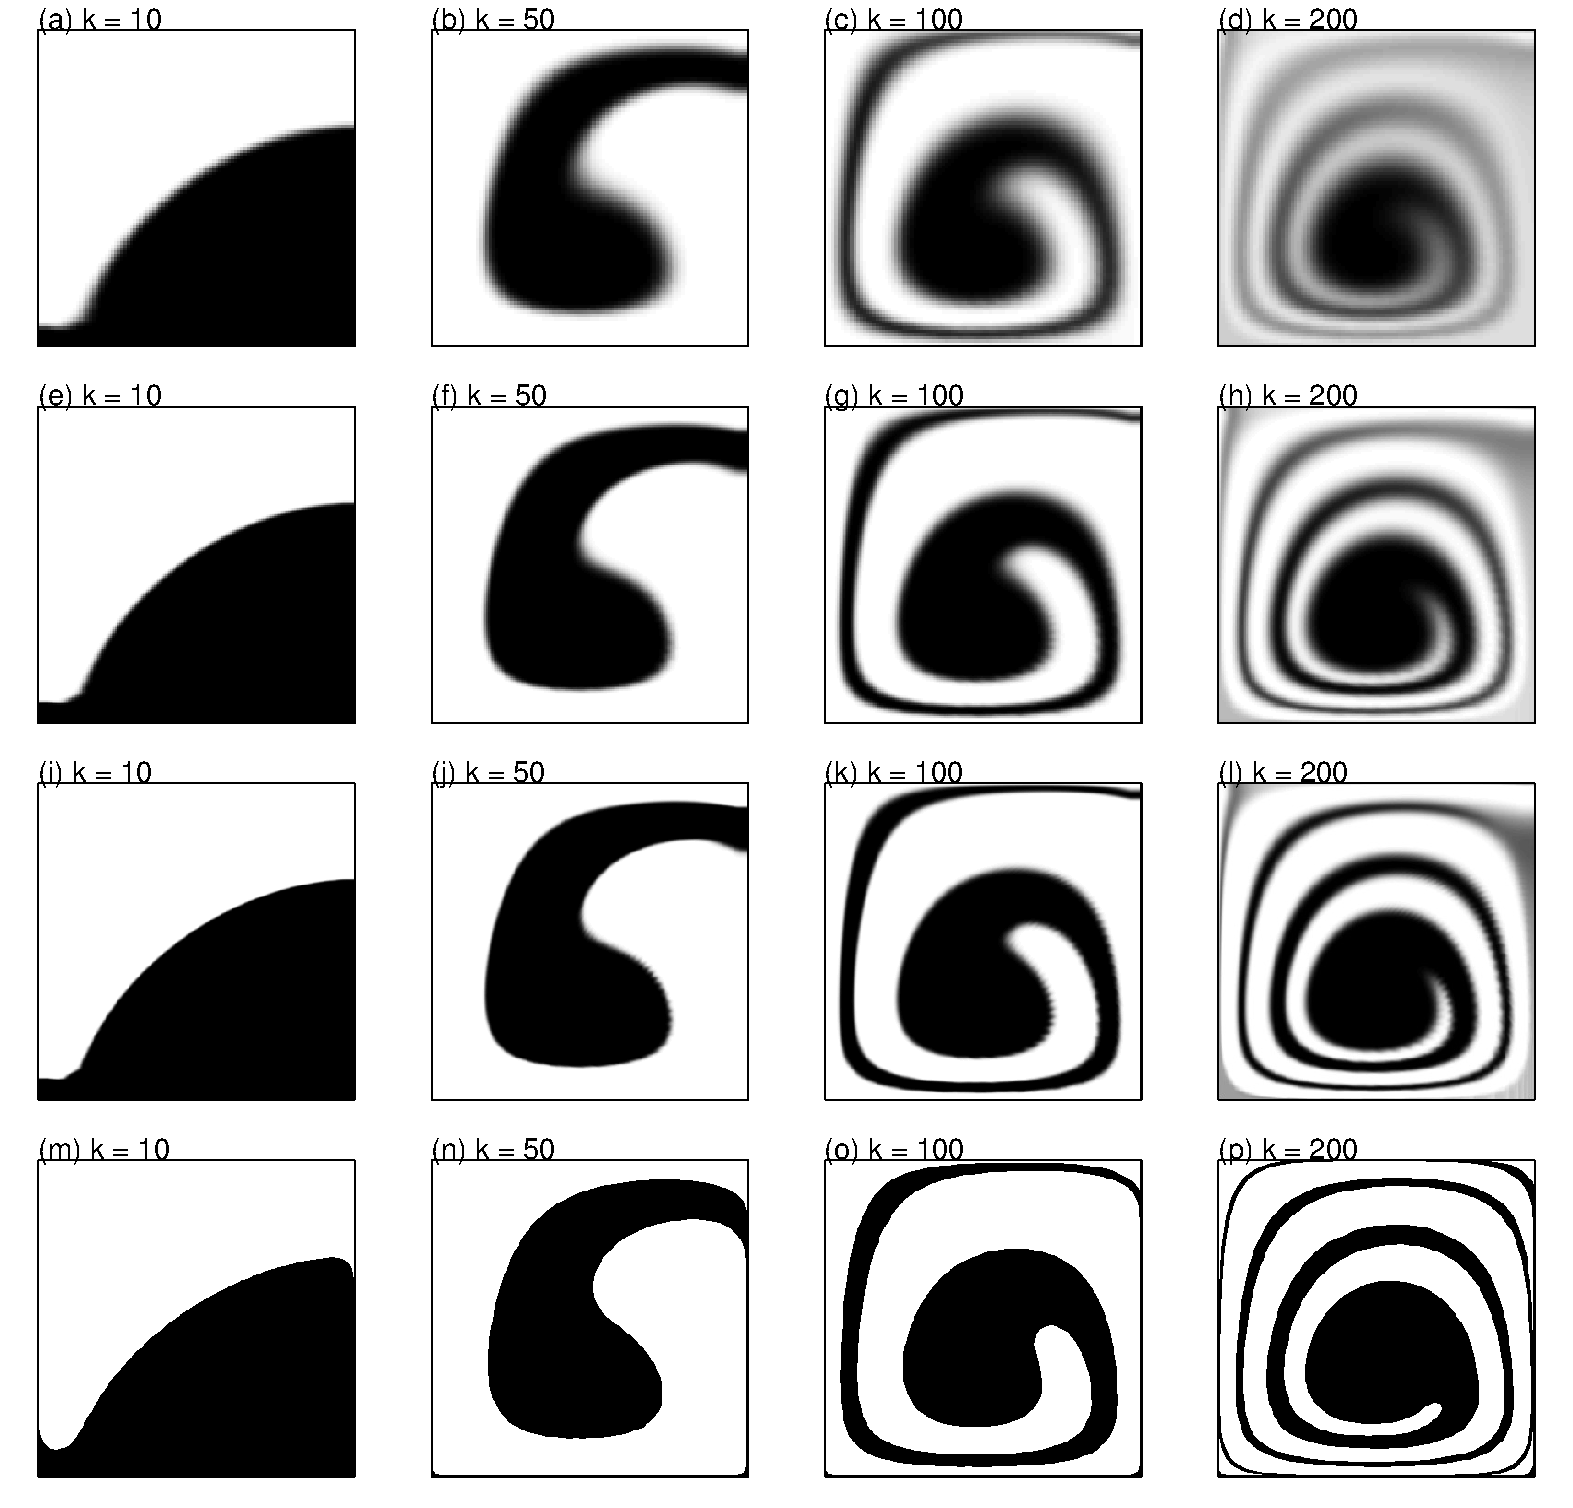
\includegraphics[width=1\textwidth]{mixingchannelcrossdiffusion}}
%  \caption{The cross-sections of the mixing channel at iterations
%    $k=10, 50, 100$, and $200$. Figures~(a)--(d) have resolution $100
%    \times 100$ ($A_{100^2}$), (e)--(h) have resolution $200 \times
%    200$ ($A_{200^2}$), and (i)--(l) have resolution $400 \times 400$
%    ($A_{400^2}$). Figures~(m)--(p) we use streamlines to evolve the
%    black/white boundary to simulate the mixing channel without any
%    diffusion.}
%  \label{mixingcrosssection}
%\end{figure}

%%%%%%%%%%%%%%%%%%%%%%%%%%%%%%%%%%%%%%%%%%%%%%%%%%%%%%%%%%
%%%%%%%%%%%%%%%%%%%%%%%%%%%%%%%%%%%%%%%%%%%%%%%%%%%%%%%%%%
\section{Results}
\label{sec:topoptresults}
%%%%%%%%%%%%%%%%%%%%%%%%%%%%%%%%%%%%%%%%%%%%%%%%%%%%%%%%%%
%%%%%%%%%%%%%%%%%%%%%%%%%%%%%%%%%%%%%%%%%%%%%%%%%%%%%%%%%%

In this section we consider four different optimized channel designs:
\begin{enumerate}
\item An interior structure to produce maximum transverse velocity:
  discussion in Section~\ref{sec:maxim-downw-veloc}, structure shown
  in Figure~\ref{example1structure}, mixing cross-sections shown in
  Figure~\ref{example1simulation}.
\item A boundary structure to produce fast mixing via alternating
  vortex pairs (a linked twist map): discussion
  in Section~\ref{sec:mixing-channel}, structure shown in
  Figure~\ref{example2structureNew} left, mixing cross-sections shown in
  Figure~\ref{example2simu}.
\item An interior structure to produce fast mixing via alternating
  vortex pairs (a linked twist map): discussion in
  Section~\ref{sec:mixing-channel}, structure shown in
  Figure~\ref{example2structureNew} right, mixing cross-sections not
  shown.
\item An interior structure to produce a transport map close to a
  rigid $45^\circ$ rotation: discussion in
  Section~\ref{sec:design-rotat-map}, structure shown in
  Figure~\ref{example3figure1}, mixing cross-sections shown in
  Figure~\ref{example3figure2}.
\end{enumerate}
Here an interior structure refers to one which can occupy some part of
the interior of the flow channel, while a boundary structure is one
that is restricted to lie within some given distance of the channel
walls. In all cases the structures were generated as described in
Section~\ref{sec:opt}, using the algorithm from
Section~\ref{sec:grad-based-optim}.

In all of our simulations, we use kinematic viscosity $\nu = 0.01 \,
\text{g} \,\text{cm}^{-1}\, \text{s}^{-1}$, cross-section dimensions
$\ell_y,\ell_z \sim 0.01\,\text{cm}$, and we adjust the body force to
make the average $x$-velocity around $1\,\text{cm}\, \text{s}^{-1}$ so
that $\text{Re} =U\ell/\nu\approx 1$.  The grid size we use to
discretize the channel cross-section is $h=1.25\times
10^{-5}\text{cm}$, which corresponds to $8 \times 10^4$ grid cells per
centimeter and a total of $M = 800 \times 800$ grid cells. The
numerical diffusion caused by this discretization is $D_{\rm num} \sim
h^2 =1.5\times 10^{-10}\,\text{cm}^2$ per period of the channel. A 2D
FFT/IFFT scheme is applied to add physical diffusion with diffusivity
$D$ at least $10^{-9}\,\text{cm}^2$ per period, and hence $D_{\rm
  num}$ is negligible.

As a guide to the order of the P\'{e}clet number $\text{Pe}$, consider
$\ell=\ell_y=\ell_z=0.01\,\text{cm}$, $\ell_x =0.02 \,\text{cm}$, $U=1
\, \text{cm} \, \text{s}^{-1}$, and take diffusivity of
$10^{-9}\,\text{cm}^2$ per period of the channel. Then $D =
10^{-9}\times U/\ell_x = 5\times10^{-8}\,\text{cm}^2\,\text{s}^{-1}$,
and $\text{Pe} = U\ell/D = 2\times10^5$. Note that the mesh we use to
solve the velocity fields ($n_x \times n_y \times n_z$) is different
from the cross-section meshes $m_y \times m_z$ used to evolve the
color fields (the latter is much higher resolution).


%%%%%%%%%%%%%%%%%%%%%%%%%%%%%%%%%%%%%%%%%%%%%%%%%%%%%%%%%%%%%%%%%%%%%%%%%%
\subsection{Maximizing the downward velocity at the center of the channel}
\label{sec:maxim-downw-veloc}
%%%%%%%%%%%%%%%%%%%%%%%%%%%%%%%%%%%%%%%%%%%%%%%%%%%%%%%%%%%%%%%%%%%%%%%%%%

This design is to demonstrate the use of the objective function of
type $g_1$ (see~(\ref{g1})) and address the porous material
regularization that we are using.

The mixing channel has dimension $(\ell_x,\ell_y,\ell_z) =
(0.02,0.01,0.01)\,$cm per period, and is discretized into
$(n_x,n_y,n_z)=(64,32,32)$ grid cells. We set $\bar{c}$ in~(\ref{g1})
to maximize the average downward (negative $y$ direction) velocity
inside the block $[0,\ell_x] \times [0.3\ell_y,0.7\ell_y] \times
[0.3\ell_z,0.7\ell_z]$. The optimization ran for $46$ iterations and
the structure shape was obtained as shown in the right of
Figure~\ref{example1structure}. Seven of the streamlines are plotted
as well. From the streamlines, it is easy to see that our objective is
achieved. In the left of Figure~\ref{example1structure} we plot how
$\bar{\alpha}$ grows versus optimization iteration number on a line
through the channel. From this plot, we see that material is initially
added in the center of the channel, but is then later removed by the
algorithm, so the gradient direction does change and we are not
solving a trivial problem. Moreover, one can clearly observe that the
material gradually forms a black/white solution such that eventually
$\bar{\alpha}$ tends to only take the value $0$ or
$\alpha_\text{max}$.

\begin{figure}
  \centerline{
    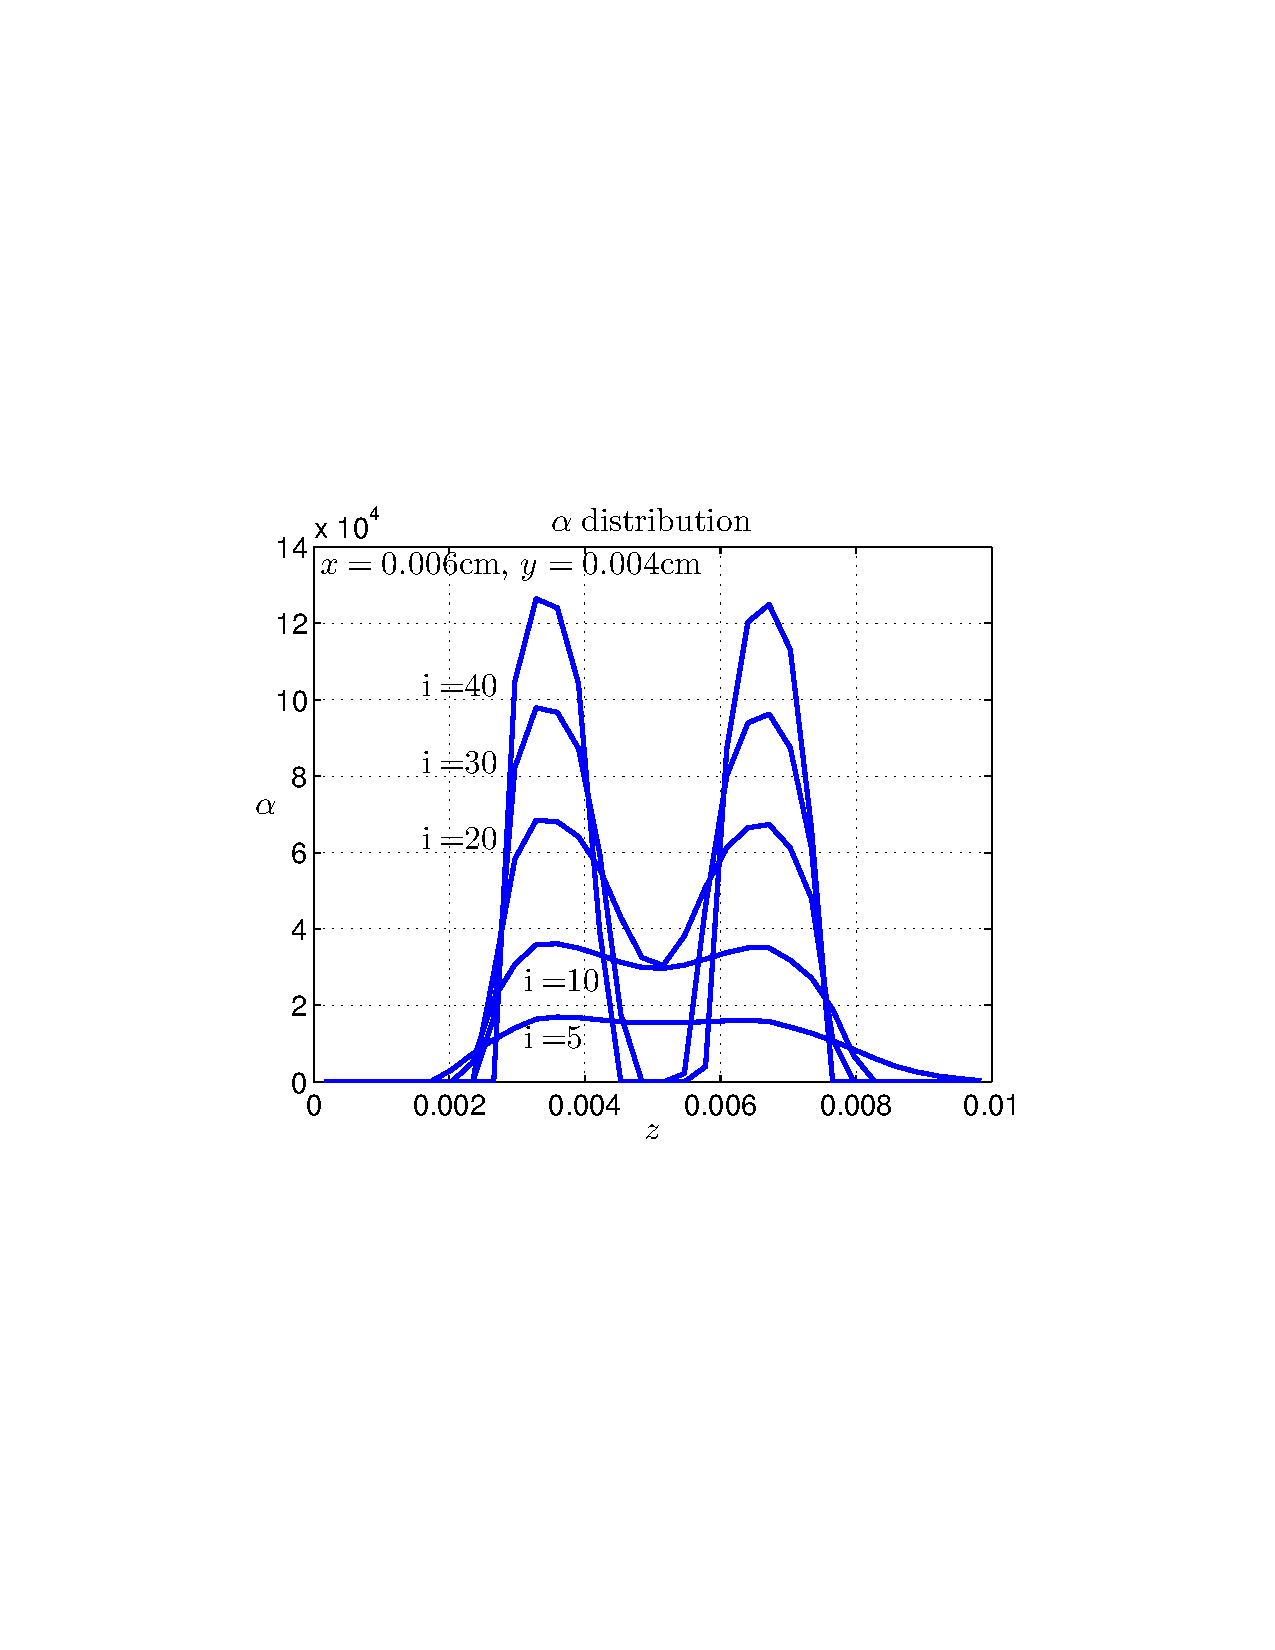
\includegraphics[width=0.5\textwidth,trim=120 240 120 240,clip=true]{example1alphaevolve}
    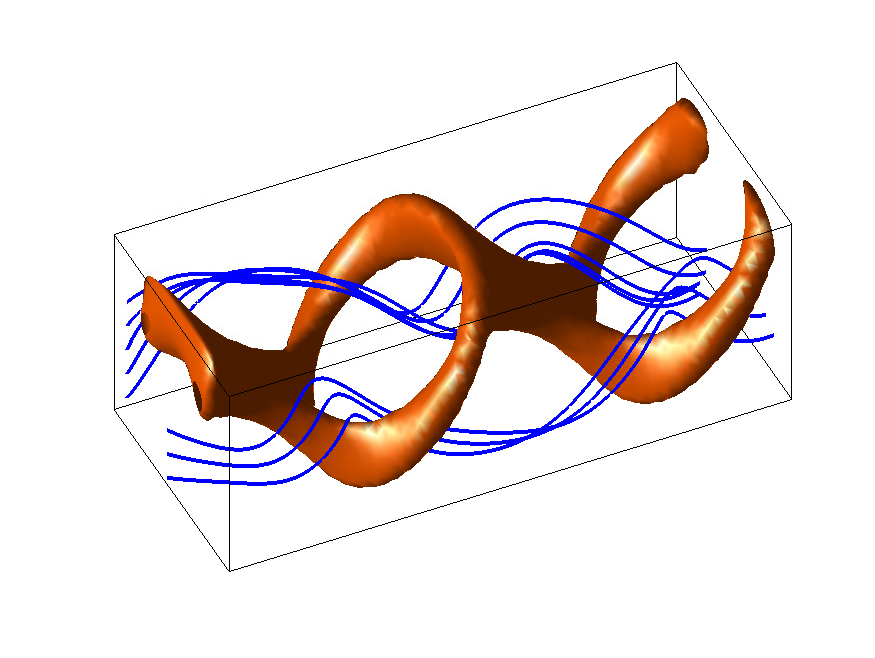
\includegraphics[width=0.5\textwidth,trim=50 20 35 30,clip=true]{example1structure2}
  }
  \caption{\label{example1structure} Optimal design for maximum
    central downward velocity (see
    Section~\ref{sec:maxim-downw-veloc}). Left: evolution of inverse
    permeability $\alpha$ versus optimization iteration number $i$,
    plotted on a vertical line in the domain. We see that material is
    initially added in the center of the channel, but is removed in
    later iterations, showing that the cost function gradient is
    changing. We also see that the optimal $\alpha$ is tending towards
    either zero or $\alpha_{\rm max}$. Right: the resulting optimal
    structure after 46 optimization iterations.}
\end{figure}

We used the simulation method discussed in Section~\ref{sec:simu} to
simulate the mixing behavior of this system. The result is shown in
Figure~\ref{example1simulation}. The system is clearly maximizing the
downward velocity at the center of the channel, as designed, which
does mix the fluid, but not as well as the designs discussed in the
next section.

\begin{figure}
  \centerline{
    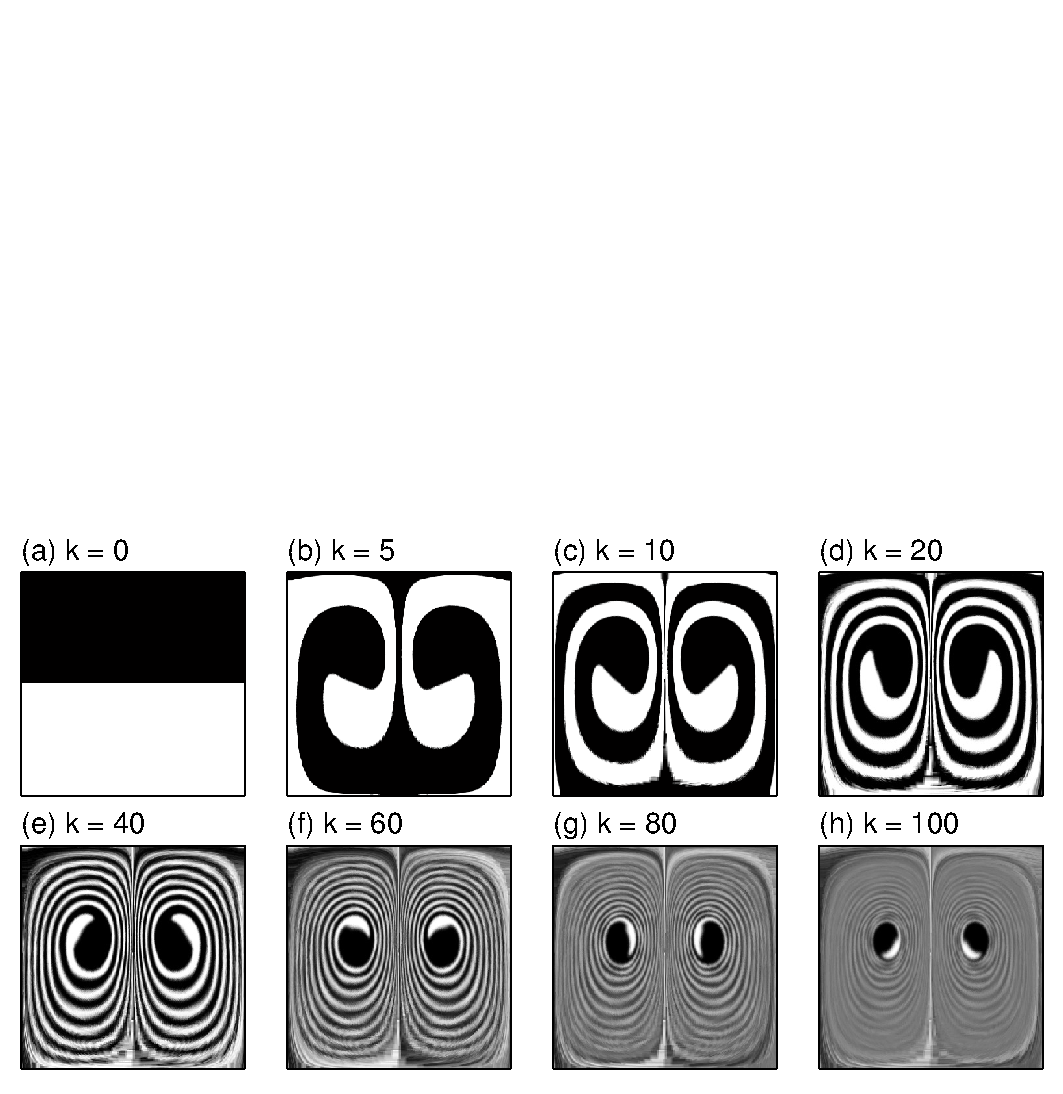
\includegraphics[width=1\textwidth,trim=0cm 0.4cm 0cm 9cm,clip]{example1simu}
  }
  \caption{\label{example1simulation} Mixing simulation for the
    maximum-downward-velocity design shown in
    Figure~\ref{example1structure} and discussed in
    Section~\ref{sec:maxim-downw-veloc}. The flow does have a very
    high downward velocity in the center, as expected.}
\end{figure}

%%%%%%%%%%%%%%%%%%%%%%%%%%%%%%%
\subsection{Designing a fast-mixing channel }
\label{sec:mixing-channel}
%%%%%%%%%%%%%%%%%%%%%%%%%%%%%%%

With this design, we want to show how the use of a $g_1$ kind of
objective function can help us to design a mixing channel to realize
fast and chaotic mixing. Stroock, et al.\ \cite{Stroock2002} proposed
a staggered herringbone mixer composed of two sequential regions of
ridges; the direction of asymmetry of the herringbones switches with
respect to the center-line of the channel from one region to the next.
The herringbone structure is fabricated with two steps of
photolithography and is located on the floor of the poly channel.
Experiments show that the length of the channel required for mixing
grows only logarithmically with $\text{Pe}$, instead of linearly as in
a smooth channel. The goal of the herringbone structure is to produce
transverse flows for which we can further optimize by the $g_1$
objective function.

The mixing channel has dimension $(\ell_x,\ell_y,\ell_z) =
(0.06,0.01,0.02)\,$cm per period and is discretized into
$(n_x,n_y,n_z)=(144,24,48)$ grids. We set $c$ to maximize the downward
(negative $y$ direction) velocity inside the offset center block
$[0,\ell_x]\times[0,\ell_y]\times[\frac{2}{6}\ell_z,\frac{5}{6}\ell_z
]$, which produces one large and one small vortex. We consider two
scenarios: (1) the material is restricted to be on the bottom of the
channel (the block $[0,\ell_x]\times[0,0.2\ell_y]\times[0,\ell_z]$) to
form a boundary structure, and (2) the material can be put anywhere
inside the channel to form an interior structure. The optimal
structures of both scenarios, as shown in
Figure~\ref{example2structureNew}, contain several periods of (almost)
the same structure. The same pattern repeats four times in the first
case and three times in the second case. One can see that in the
first case, the optimal structure is also a herringbone type, but
has a higher frequency for the smaller vortex. For the second
scenario, the structure is formed by much more material and also tends
to have a higher frequency for the smaller vortex.

We emphasize that in both designs the initial structure state was
$\bar{\alpha} = 0$, so the formation of the herringbone pattern is
entirely driven by the optimization algorithm. Interestingly, it
appears to be more efficient to have asymmetric frequencies for the
herringbone structure. The choice of domain size that we used for
optimization (in particular $\ell_x$) does determine the herringbone
frequency, as an integer number of structures must fit within this
periodic domain.

Just like in the previous example, one can simulate how the channel
mixes the colors by the Markov Chain model. However, in order to
produce chaotic mixing, the mixer has to be composed of two sequential
regions that are symmetric with respect to the plane
$z=\frac{1}{2}\ell_z$, and this breaks the periodic boundary condition
assumed in obtaining the Markov Chain. In order to perform a correct
simulation, we need to solve the flow field for a full cycle of
channel.

Let us focus on the first scenario. Since the same structure repeats
four times in the solution, we take one of them and call it ``L''
(with dimension $(\ell_x,\ell_y,\ell_z)=(0.015,0.01,0.02)\,)$cm. The
symmetric structure of ``L'' is thus called ``R''. We can build an
$n$-cycle channel by connecting $n/2$ L structures and $n/2$ R
structures together. It thus has the period $0.015n\,\text{cm}$. For
fixed $\text{Pe}=1.2 \times 10^4$, we solve the flow field for
different $n$-cycles with $n=6$, $8$, $10$ and $12$, and find that
when $n=8$, the channel has the best mixing. Hence in
Figure~\ref{example2trajectory}, the 8-cycle mixing channel is used to
perform the simulation with different $\text{Pe}$. We adjust
$\text{Pe}$ by changing the FFT/IFFT diffusivity between each
$8$-cycle ($0.12\,\text{cm}$). The trajectories have the same tendency
as the experiment results in Figure~3(D) in \cite{Stroock2002}.  We
define the mixing length $x_{90}$ as the channel length required for
the standard deviation to drop to $0.05$ (shown by a dashed line in
Figure~\ref{example2trajectory}). We see that the mixing length grows
linearly with $\log(\text{Pe})$, which matches the experimental
results~\cite{Stroock2002}.

In Figure~\ref{example2simu} we show cross-sectional plots of two of
the simulations in Figure~\ref{example2trajectory}, where the channel
is an 8-cycle and $\text{Pe}$ is $1.2\times10^6$ (left column) and
$1.2\times10^9$ (right column). The first four rows show the
cross-sections at the end of the 1st to the 4th cycle, and the last
row shows the cross-sections at the end of the 9th cycle. From this
comparison we can clearly see how the chaotic mixing protocol enhances
mixing even when diffusion is very small.

As for the 3D structure, the best $n$-cycle we founds was $n=2$
($\ell_x=0.04\, \text{cm}$), because this structure stirs the flow a
great deal.  To further compare our optimized structures and the
design in \cite{Stroock2002}, we also performed a simulation of
Stroock's staggered herringbone mixer. The mixing length versus
$\log({\text{Pe}})$ for the three simulations and the experiment data
given in \cite{Stroock2002} are plotted in
Figure~\ref{example2mixinglength}. We see that our simulation
($\times$) of Stroock's design has a slightly longer mixing length
than the experiment data ($\lozenge$) when $\text{Pe}$ is small, and
they agree well when $\text{Pe}\approx 10^6$
($\log(\text{Pe})=14$). As for our optimal mixing channel designs
($\square$ for the herringbone, and $\bigcirc$ for the 3D
structures), they both significantly outperform Stroock's design in
our simulations. To quantify this improvement, consider $\log(Pe) =
12$, where $x_{90}$ is reduced from $1.5\,\text{cm}$ (Stroock's
herringbone) to $1.0\,\text{cm}$ (optimal herringbone) or
$0.6\,\text{cm}$ (optimal 3D structure). The optimized channels thus
have improvements of 30\% and 60\%, respectively, in mixing lengths.

We emphasize that we are not directly optimizing the mixing rate of
the channel. Instead, only the proxy cost function $g_1$ is being
optimized, to produce higher downward velocities at the offset point
in the channel. These results thus indicate that this is a reasonable
function to optimize when the goal is fast mixing, as it is producing
a channel with a linked-twist-type structure with strong twisting for
a short channel length.

In Figure~\ref{example2crosscompare}(a) and (b) we plot the
cross-section at the end of the $5$-th cycle of our optimal
herringbone solution and Stroock's design, for
$\log(\text{Pe})=14$. We can compare the simulation in
Figure~\ref{example2crosscompare}(b) with Figure~3(C) in
\cite{Stroock2002} to see how similar they are.  This suggests that
our approximate Markov Chain mixing model is indeed valid when the
diffusion is small.

For the above two cases, the average flow velocity in the $x$
direction is around $1.2\, \text{cm} \,\text{s}^{-1}$. We use the same
body force for the simulation of the optimal 3D structure, and
adjust the diffusivity to make $\log(\text{Pe})=14$. The optimal 3D
structure has a much shorter cycle length
($\ell_x=0.04\,\text{cm}$). Hence we plot the cross-section of it at
the end of $15$-th cycle in Figure~\ref{example2crosscompare}(c). It
shows that when $x=0.6\, \text{cm}$, the mixing is stronger than
either herringbone type channel. However, since there is more material
inside the channel, for the same body force, the average flow velocity
in the 3D structure channel is only $0.2\, \text{cm}
\,\text{s}^{-1}$---six times slower than the herringbone type
channels. Hence when we plot the cross-section of this mixing channel
at time $t=0.7s$ in Figure~\ref{example2crosscompare}(d), it is not
significantly better than the other two channels at $t=0.5\,s$ and
$t=0.6\,s$. This means that if we care more about mixing time rather
than mixing length, or if the available pressure is limited, then the
3D structure may not be the preferable choice.

%%%%%%%%%%%%%%%%%%%%%%%%%%%%%%%%%%%%%%%%%%%%%%
% structure plot
  \begin{figure}
    \centerline{
      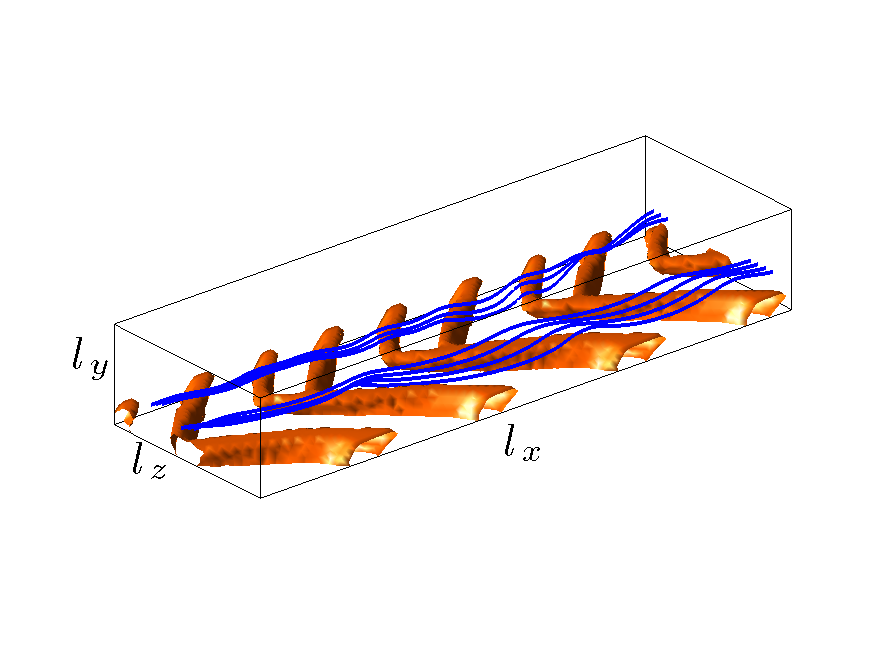
\includegraphics[width=0.5\textwidth,trim=35 75 35 65,clip=true]{example2structureherringbone}
      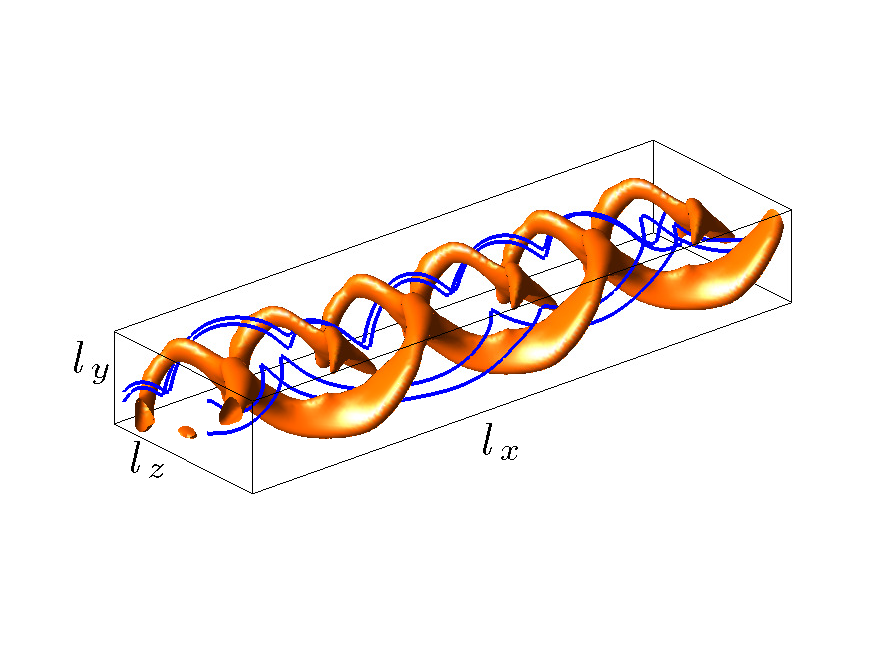
\includegraphics[width=0.5\textwidth,trim=35 75 35 65,clip=true]{example2structure3d}
     %\scalebox{0.6}[0.6]{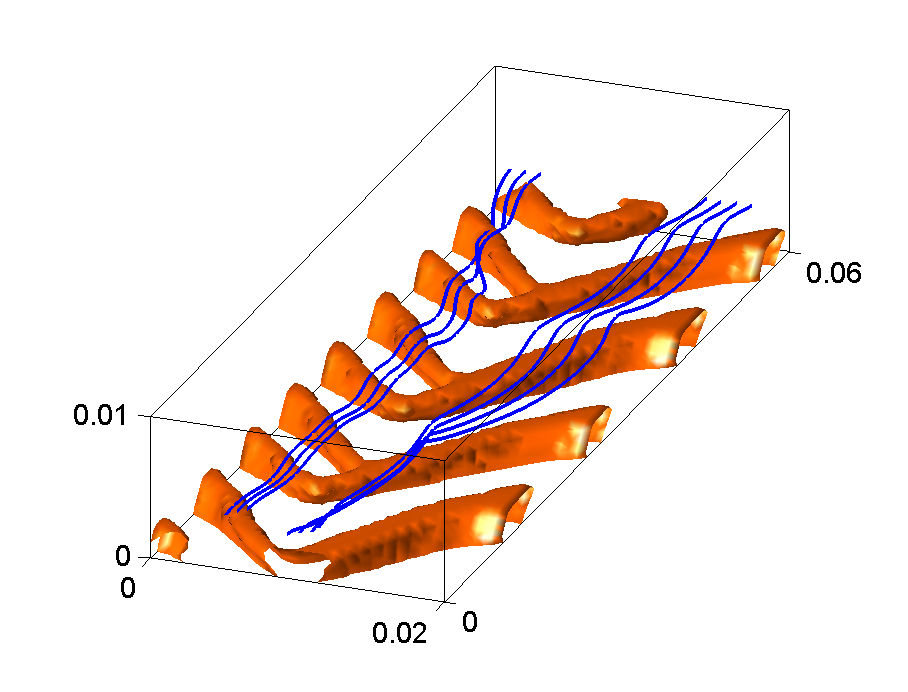
\includegraphics{myharringbonestructure}}
     %\scalebox{0.6}[0.6]{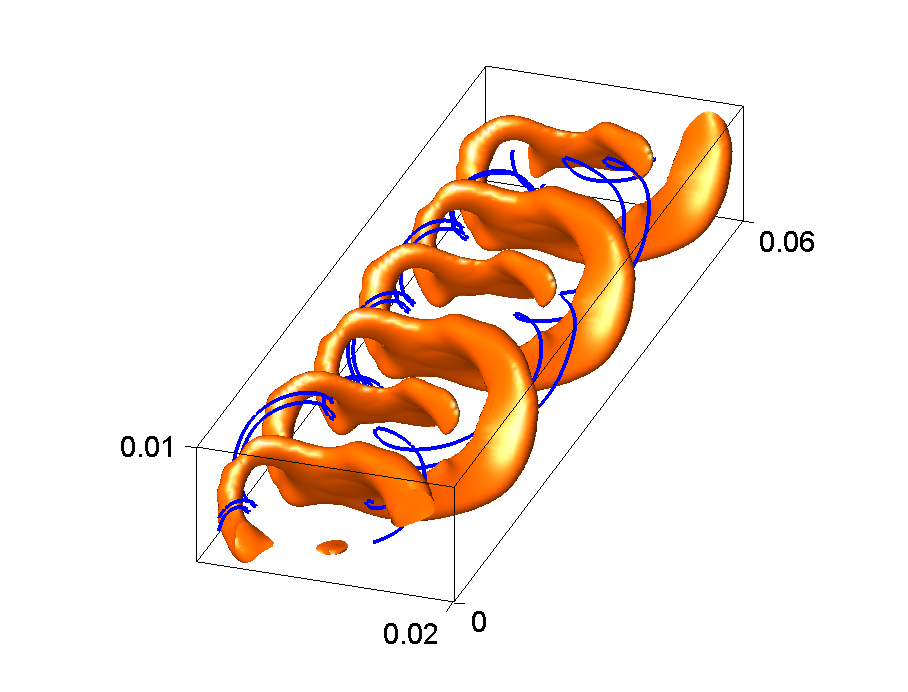
\includegraphics{my3dstructure}}
      }
      \caption{\label{example2structureNew} Optimal channel structures
        for fast mixing (see Section~\ref{sec:mixing-channel}), with a
        pair of asymmetric vortices. Left: boundary optimal solution
        with material restricted to lie only in a region near the
        boundary. Right: interior optimal solution with no
        restrictions on material placement.}
  \end{figure}
%%%%%%%%%%%%%%%%%%%%%%%%%%%%%%%%%%%%%%%%%%%%%%%

%%%%%%%%%%%%%%%%%%%%%%%%%%%%%%%%%%%%%%%%%%%%%%%
%mixing trajectory
  \begin{figure}
    \centerline{
     %\scalebox{0.5}[0.5]{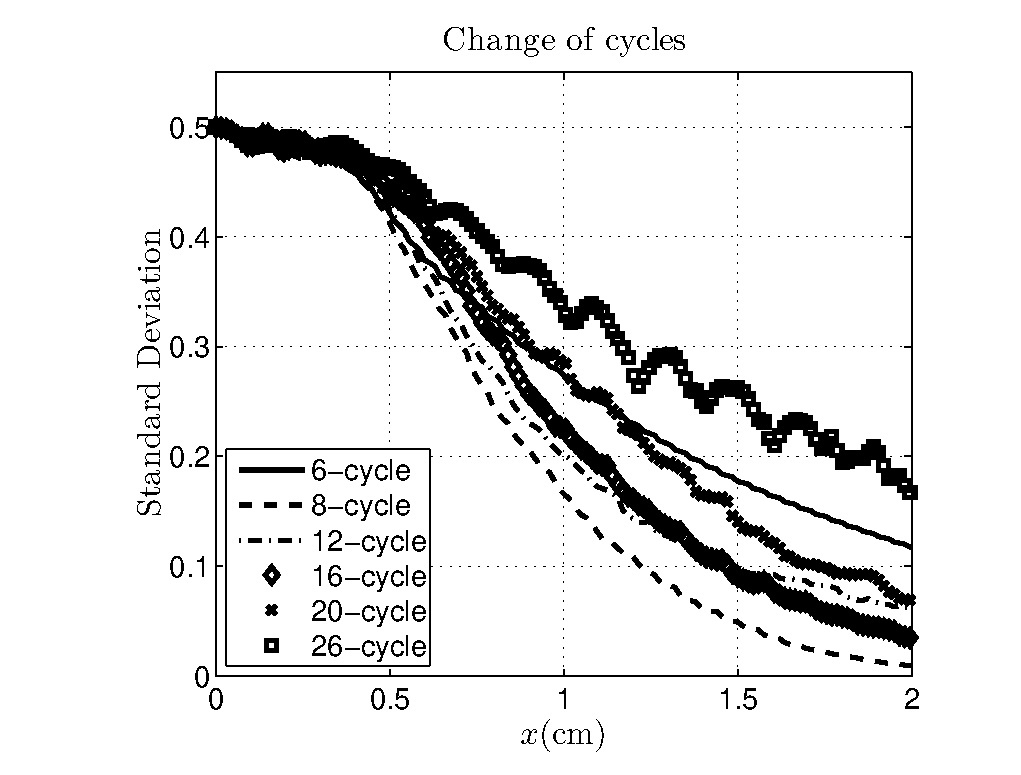
\includegraphics{example2veryCycles}}
      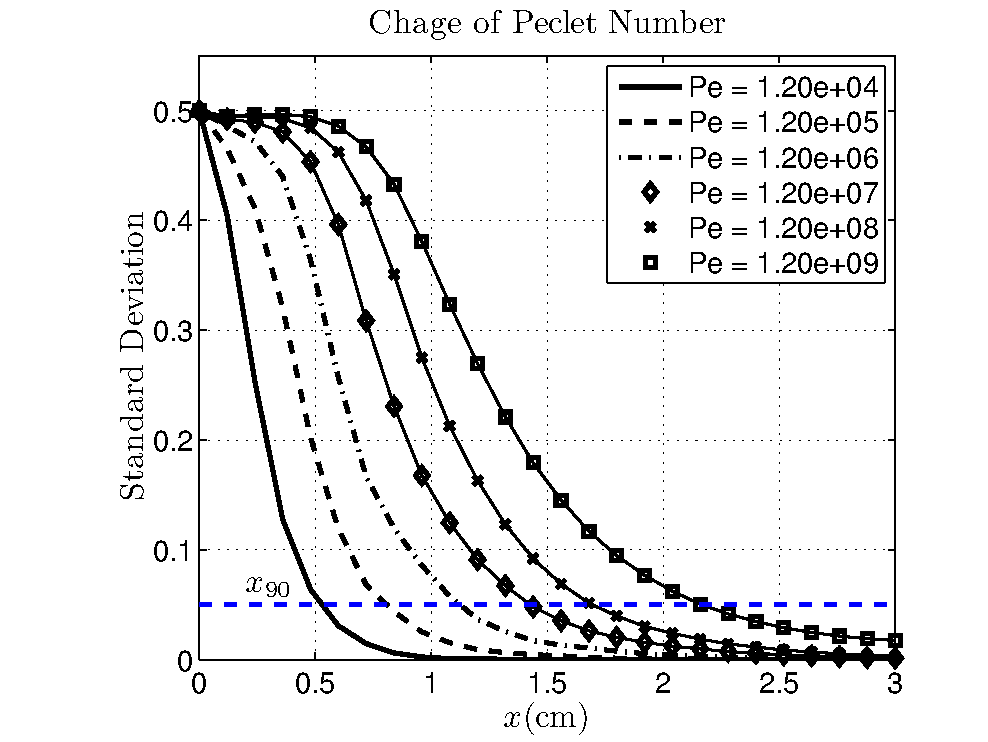
\includegraphics[width=0.5\textwidth,trim=50 0 30 20,clip=true]{example2veryPe2}}
    \caption{\label{example2trajectory} Variation of mixing (standard
      deviation of color field $f$) with distance downstream and
      influence of changing diffusivity $D$ and hence changing
      P\'{e}clet number Pe, for the $8$-cycle optimal herringbone
      structured channel (see Section~\ref{sec:mixing-channel} and
      Figure~\ref{example2structureNew} left).}
  \end{figure}
%%%%%%%%%%%%%%%%%%%%%%%%%%%%%%%%%%%%%%%%%%%%%%%

%%%%%%%%%%%%%%%%%%%%%%%%%%%%%%%%%%%%%%%%%%%%%%%
%cross-section simulation 1, for different Pe
  \begin{figure}
    \centerline{
      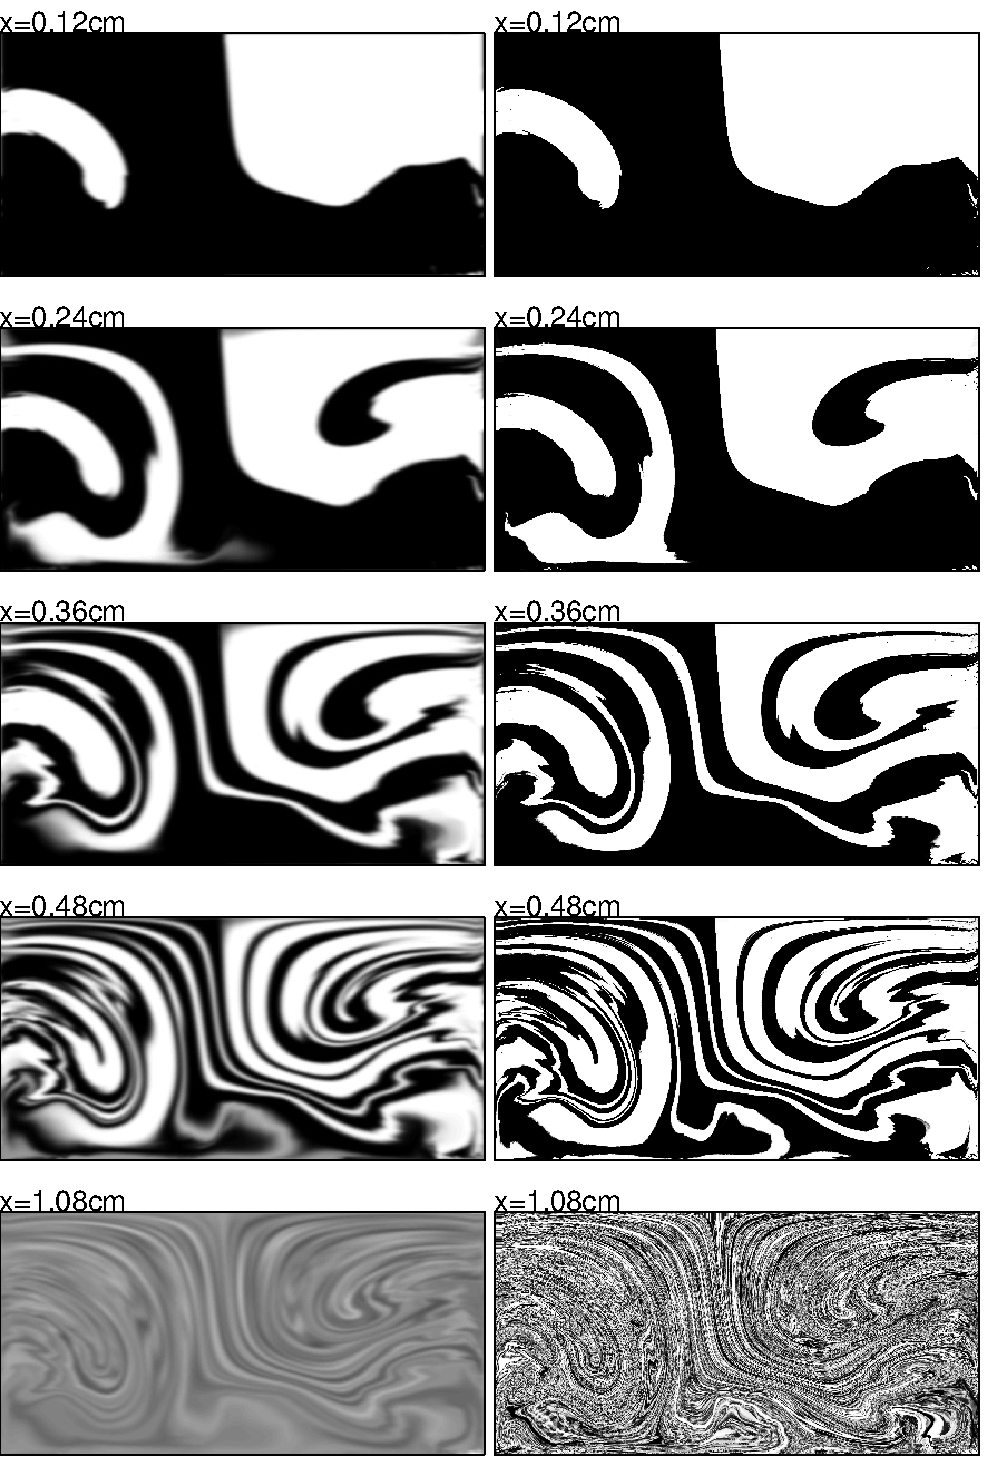
\includegraphics[width=0.6\textwidth]{example2simu2}
    }
    \caption{\label{example2simu} Mixing cross-sections for the
      $8$-cycle optimal herringbone structured channel (see
      Section~\ref{sec:mixing-channel} and
      Figure~\ref{example2structureNew} left), for $\text{Pe} =
      1.2\times10^6$ (left) and $1.2\times10^9$ (right). The first
      four rows show cross-sections after 1 to 4 cycles, while the
      last row shows cross-sections after , we plot the cross-sections
      of the end of the 1st to the 4th cycle for both cases. The
      bottom two plots show the cross-sections of the end of the 9th
      cycle for both cases. We see that mixing is occurring even with
      very small diffusivity.}
  \end{figure}
%%%%%%%%%%%%%%%%%%%%%%%%%%%%%%%%%%%%%%%%%%%%%%%

%%%%%%%%%%%%%%%%%%%%%%%%%%%%%%%%%%%%%%%%%%%%%%%%
% mixing length vs Pe, 4 cases
  \begin{figure}
    \centerline{
      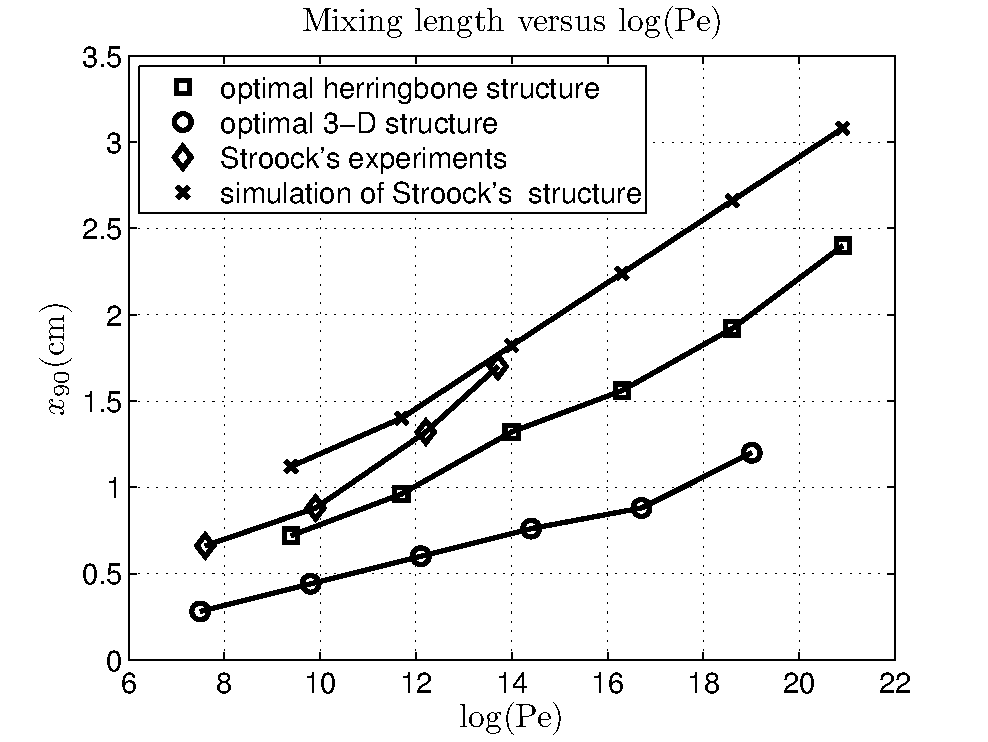
\includegraphics[width=0.58\textwidth,trim=10 0 10 22,clip]{example2mixinglength2}
    }
    \caption{\label{example2mixinglength} Mixing length $x_{90}$
      versus P\'eclet number for fast-mixing channel designs. We see
      that our numerical results ($\times$) agree reasonably well with
      experiments ($\lozenge$). Comparing numerical simulations, the
      optimal boundary herringbone structure ($\square$) is superior
      to the Stroock structure ($\times$), while the optimal interior
      3D structure ($\circ$) is the best.}
  \end{figure}
%%%%%%%%%%%%%%%%%%%%%%%%%%%%%%%%%%%%%%%%%%%%%%%%

%%%%%%%%%%%%%%%%%%%%%%%%%%%%%%%%%%%%%%%%%%%%%%%%
% cross-section comparison for 3 cases.
  \begin{figure}
    \centerline{
      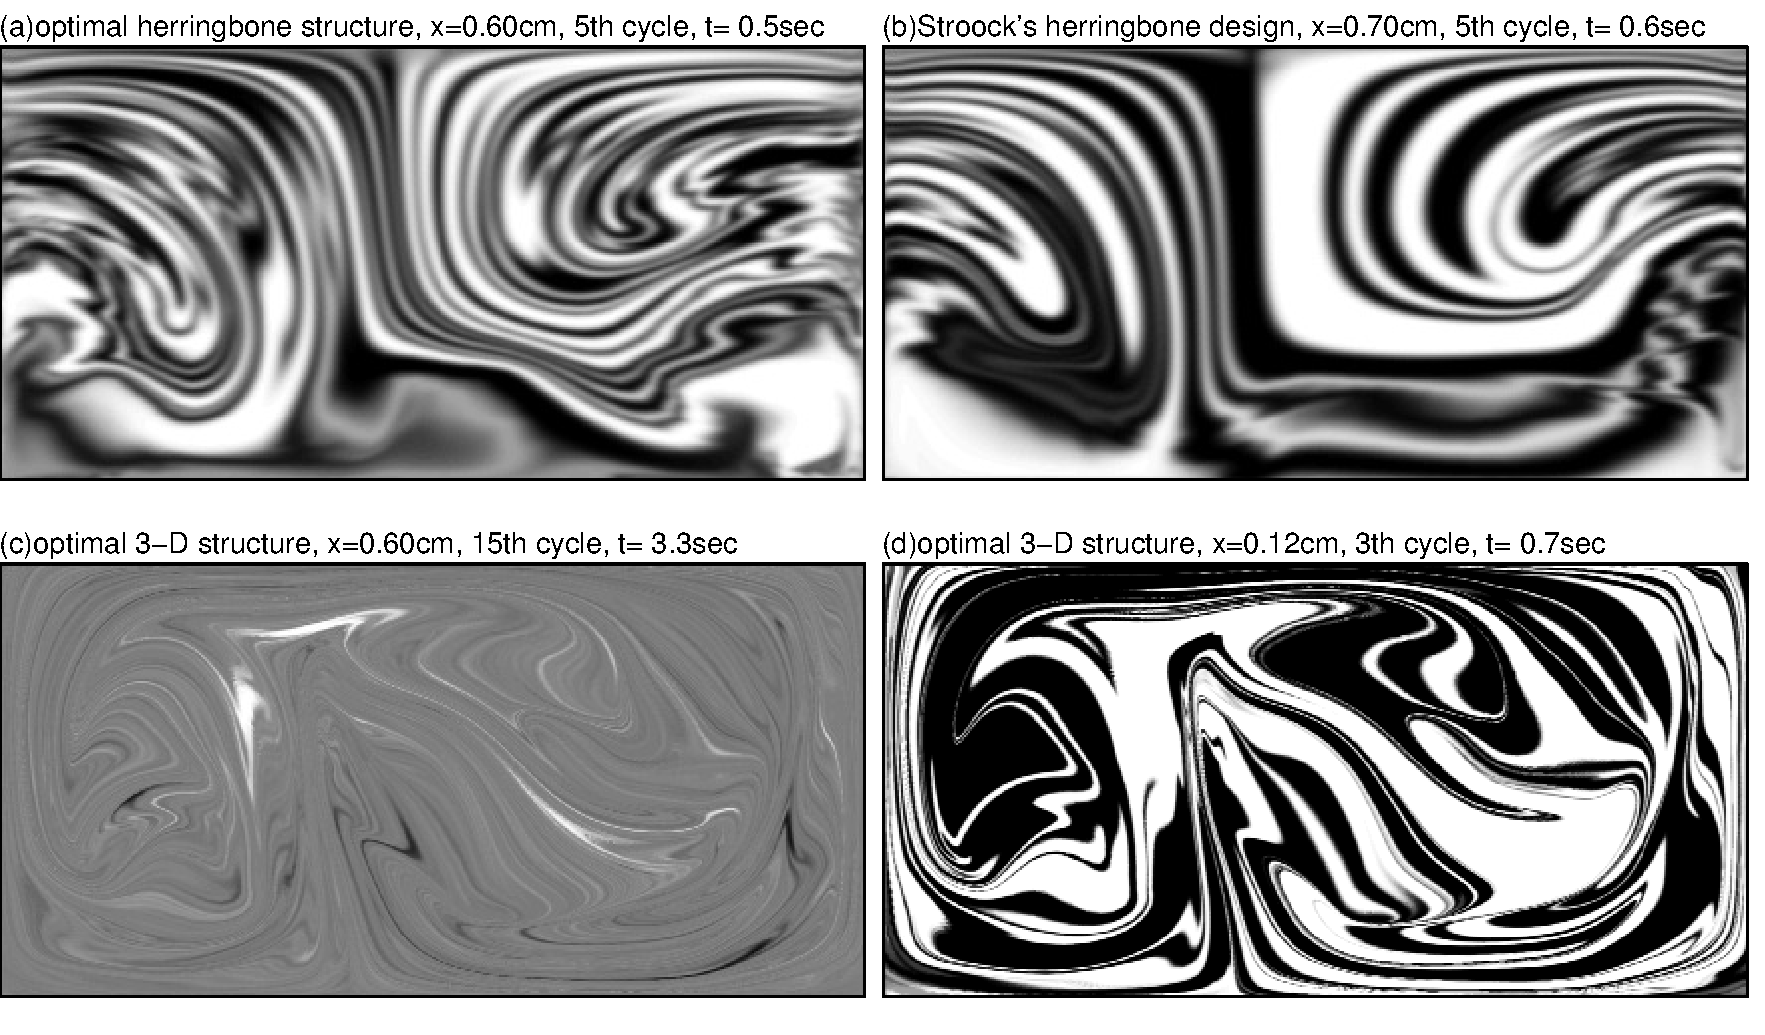
\includegraphics[width=1\textwidth,trim=0 20 7 5,clip=true]{example2crosscompare}
    }
    \caption{\label{example2crosscompare} Mixing cross-sections for
      the fast-mixing designs: (a) the optimal herringbone structure
      at the end of its $5$th cycle; (b) the simulation of Stroock's
      herringbone design at the end of its $5$th cycle; (c) the
      optimal 3D structure at the end of its $15$th cycle; and (d)
      the optimal 3D structure at the end of its $3$th cycle. The
      color distribution in (b) is almost the same as the experimental
      result shown in Figure~3(C) in \cite{Stroock2002}, validating
      the numerical results.  Plots (c) and (d) show that although the
      3D structure has a much smaller mixing length ($x_{90}$), it
      also slows the flow much more. For the same body force, the
      average velocity in the $x$-direction is only $1/6$ of that for
      the herringbone type structures. Hence for the same body force
      and the same mixing time, the 3D structure is not better than
      the optimal herringbone structure.}
  \end{figure}
%%%%%%%%%%%%%%%%%%%%%%%%%%%%%%%%%%%%%%%%%%%%%%%%

%%%%%%%%%%%%%%%%%%%%%%%%%%%%%%%
\subsection{Designing a rotation map}
\label{sec:design-rotat-map}
%%%%%%%%%%%%%%%%%%%%%%%%%%%%%%%

The channel designs in previous sections all used linear cost
functions $g_1$ to optimize fluid velocity at certain points in the
channel. In this section we demonstrate how the cost function $g_2$
in~(\ref{g2}) can be used to design channel that produces a given
transport map $S^*$, using a test case of a twist map, as would be
used to implement a linked twist mixer~\cite{Wiggins2004}.

There are various kinds of twist maps, for example,
$S^* : (y,z) \mapsto (y_e,z_e)$, for
\begin{align*}
   y_e &= y_c + r \cos(\alpha+\theta), \\
   z_e &= z_c + r \sin(\alpha+\theta), 
 \intertext{where}
   \alpha &= \text{atan2}(y-y_c,z-z_c), \\
   r      &= \sqrt{(y-y_c)^2 +(z-z_c)^2}.
\end{align*}
This defines a twist map centered at $(y_c,z_c)$ with a fixed angle of
rotation $\theta$. This is not a realistic map for a channel because
it does not satisfy the non-slip boundary conditions on the
walls. Nonetheless, we use this as our desired map $S^*$, with the
understanding that our optimized $S$ map will only approximate $S^*$
near the channel center. Again, the mixing channel has dimension
$(\ell_x,\ell_y,\ell_z) = (0.02,0.01,0.01)\,$cm per period, and is
discretized into $(n_x,n_y,n_z)=(64,32,32)$ grid cells. We use the
objective function $g_2$ from~(\ref{g2}) for the above desired map and
set $(y_c,z_c) =(0.5\ell_y, 0.5\ell_z)$ and $\theta = 45^\circ$.

The structure after $40$ optimization iterations is shown on the left
of Figure~\ref{example3figure1}. A set of streamlines starting from
$41 \times 41$ regular grid points are calculated, and the end points,
which form the twisted grid, are plotted on the right of
Figure~\ref{example3figure1} overlaying the original grid. The
extra-thick line shows a block whose edges are originally parallel to
the channel walls and now rotated almost $45^\circ$. In
Figure~\ref{example3figure2} we show the mixing cross-sections of this
channel. In the first 7 periods we can see how it rotates the
boundary between the colored liquids by roughly $45^\circ$ each period. The last
plot in Figure~\ref{example3figure2} shows the color field at the
$100$th iteration.

Obviously, this channel does a bad job in mixing, but it is possible
that this design route could lead to suitably offset twist maps that
could be combined into an efficient mixing channel.

Interestingly, unlike the optimal channel designs found in
Sections~\ref{sec:maxim-downw-veloc} and~\ref{sec:mixing-channel}, the
optimal structure for this design is not solid. That is, the optimal
$\alpha$ has values between 0 and $\alpha_{\rm max}$. To actually
fabricate this structure, a porous material would be needed.

\begin{figure}
  \centerline{
    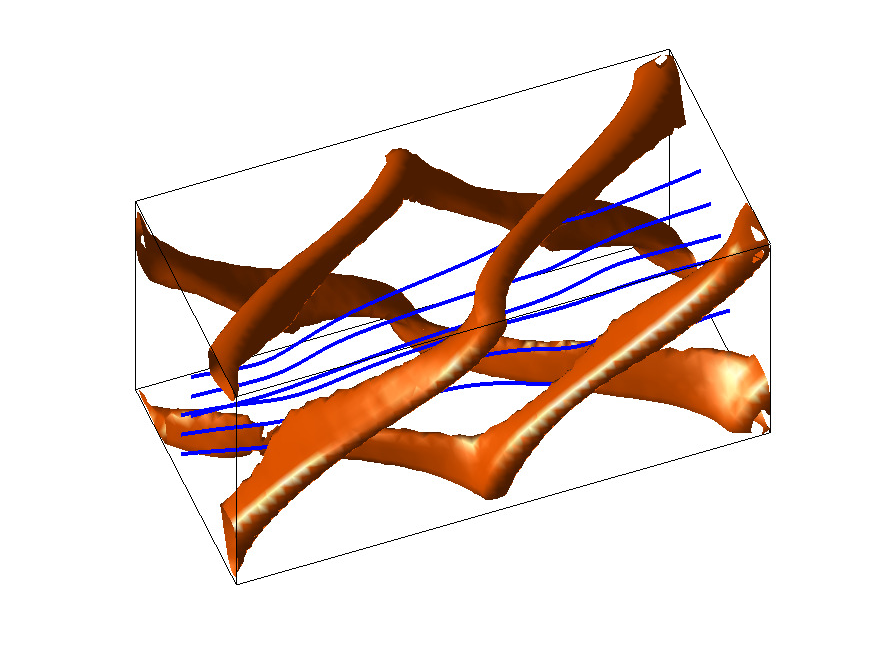
\includegraphics[width=0.5\textwidth,trim=60 30 50 20,clip]{example3structure}
    \hfill
    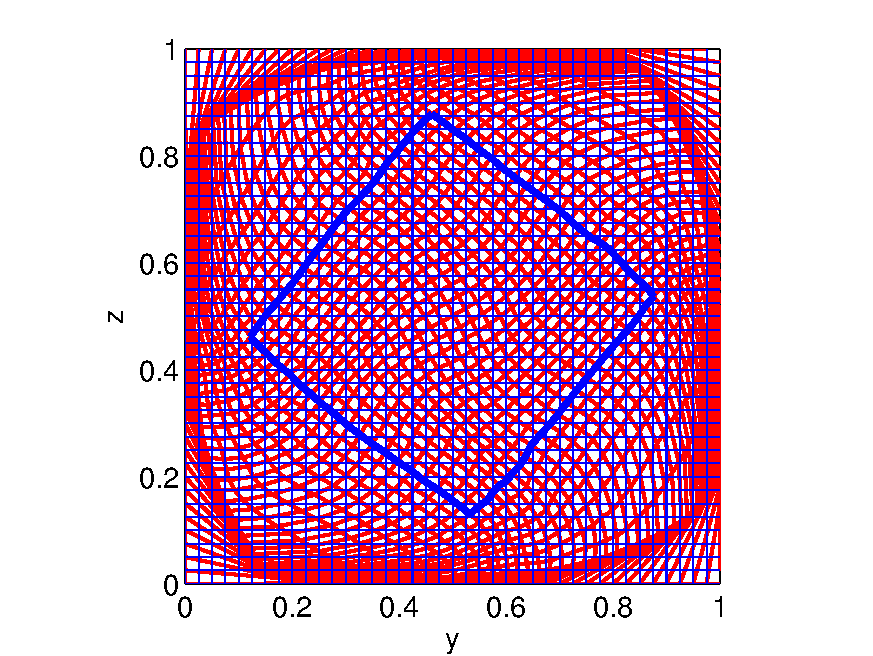
\includegraphics[width=0.45\textwidth,trim=50 0 60 20,clip]{example3grid}}
  \caption{\label{example3figure1} Optimal structure to twist the flow
    by $45^\circ$. Left: structure and streamlines (note that the
    structure is not solid, but is porous, unlike all other optimal
    structures in this paper). Right: particle transport map for one
    period of this structure, with a regular grid and its image
    overlaid. A thick line shows the image of a square whose edges
    were originally parallel to the boundary, but is now rotated by
    $45^\circ$ as desired. The non-slip boundary conditions means that
    this map is not a rigid rotation near the boundary.}
\end{figure}


\begin{figure}
  \centerline{
    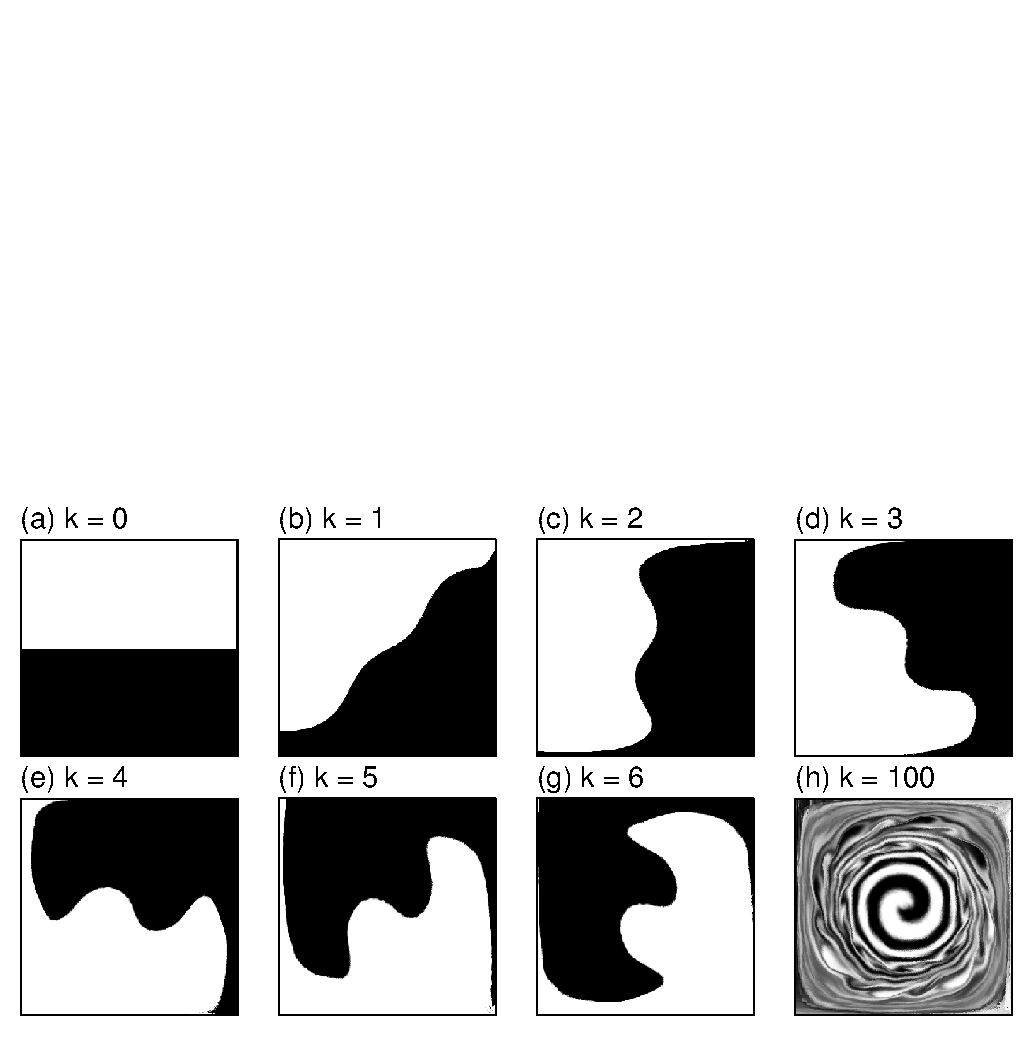
\includegraphics[width=0.9\textwidth,trim=0.2cm 0.2cm 0.2cm 8.5cm,clip]{example3simu}}
  \caption{\label{example3figure2} Mixing cross-sections for the
    rotating channel design shown in Figure~\ref{example3figure1}. For
    the first $6$ periods, the flow field is approximately rotated
    $45$ degrees per period. The last plot shows the cross-section at
    the $100$th iteration.}
\end{figure}


%%%%%%%%%%%%%%%%%%%%%%%%%%%%%%%%%%%%%%%%%%%%%%%%%%%%%%%%%%
%%%%%%%%%%%%%%%%%%%%%%%%%%%%%%%%%%%%%%%%%%%%%%%%%%%%%%%%%%
%
% Conclusion
%
\section{Conclusion}
\label{sec:topoptconclusion}

We have demonstrated a topology optimization method to design the flow
field of a periodic microfluidic channel, using the relaxation
\cite{Evgrafov2005, Borrvall2003} of Stokes flow in an irregular
geometry to Darcy flow with porous material. The objective function
can be either a function of velocity components or a distance between
inlet-outlet flow maps, and the optimization uses gradient descent
with adjoint method gradient calculation. We also developed a
probabilistic model to approximate the solution of the
advection-diffusion equation on the cross-sections of the mixing
channel. We demonstrated the feasibility of this model by reproducing
the experimental results given in \cite{Stroock2002} with reasonable
accuracy. Using our topology optimization method, we presented
improved mixing channel designs that reduce the mixing length by 30\%
(optimal herringbone) and 60\% (optimal 3D structure). Of course,
these results are only in simulation and may not be reflected by
experimental implementations.

Although it may be possible to improve mixing rates by designing flow
maps, such as twist maps, it is possible that the resulting channel
structures will be porous, as we saw in
Section~\ref{sec:design-rotat-map}. Such channels may pose fabrication
challenges, making them infeasible in practice.

While we have optimized proxy cost functions, such as downward
velocities at certain points, it would be attractive to directly
optimize mixing. This could possibly be done by taking the cost
function to be the variance or mix-norm \cite{Mezic2005} of a color
field after a certain channel length, for example, although the
efficient computation of gradients could present challenges.

One choice of cost function which might seem appealing, but which we
believe does not work in practice, is the second largest eigenvalue
modulus (SLEM) \cite{Boyd2004} of the approximate advection map
$U_{S^{-1},n}$. While minimizing the SLEM does maximize the worst-case
long-time mixing over all inlet color distributions, we are much more
concerned with particular initial conditions (poorly mixed ones) and
the initial transient mixing behavior.

In fact, the transient phenomena may be unrelated to the eigenvalues
of $U_{S^{-1},n}$, and have nontrivial relation to the pesudospectra
\cite{Lloyd2005}. Perhaps the famous examples feature the so-called
``cutoff phenomenon'' in finite Markov Chains \cite{Diaconis1996,
  Diaconis2005, LSaloff-Costt2004}, which have interesting connections
with chaotic mixing \cite{numcutoff, symdyn}.

The mixing behavior of the fast-mixing channels shown in
Figure~\ref{example2trajectory} show cutoff-type behavior: as
$\text{Pe}$ becomes larger, the standard deviation initially stays
high for a longer time before dropping rapidly. So even though the
mixing length grows logarithmically with $\text{Pe}$, for a fixed Pe
we cannot halve the channel length and expect to see half the
mixing. Instead, for a given Pe, there is a certain channel length
necessary to have reasonable mixing. A too-short channel may produce
almost no mixing, while a too-long channel is unnecessary.

Such multi-stage mixing trajectories have been widely observed and
studied in chaotic map mixing: see \cite{Thiffeault2003-13,
  Thiffeault2003-309, Thiffeault2004, Tsang2005, Haynes2005} for
examples. In \cite{numcutoff}, the authors study the standard map with
small diffusion, and show how the multi-stage mixing behavior of this
chaotic map is related to the cutoff phenomenon for Markov chains.

%%%%%%%%%%%%%%%%%%%%%%%%%%%%%%%%%%%%%%%%%%%%%%%%%%%%%%%%%%
%%%%%%%%%%%%%%%%%%%%%%%%%%%%%%%%%%%%%%%%%%%%%%%%%%%%%%%%%%

% References
%\bibliographystyle{plain}
 \bibliographystyle{wileyj}
\bibliography{../mixingbib}


\end{document}
